\documentclass[12pt]{beamer}
\usepackage{../Estilos/BeamerMAF}
\usepackage{../Estilos/ColoresLatex}
%Sección para el tema de beamer, con el theme, usercolortheme y sección de footers
\usetheme{CambridgeUS}
\usecolortheme{beaver}
%\useoutertheme{default}
\setbeamercovered{invisible}
% or whatever (possibly just delete it)
\setbeamertemplate{section in toc}[sections numbered]
\setbeamertemplate{subsection in toc}[subsections numbered]
\setbeamertemplate{subsection in toc}{\leavevmode\leftskip=3.2em\rlap{\hskip-2em\inserttocsectionnumber.\inserttocsubsectionnumber}\inserttocsubsection\par}
\setbeamercolor{section in toc}{fg=blue}
\setbeamercolor{subsection in toc}{fg=blue}
\setbeamercolor{frametitle}{fg=blue}
\setbeamertemplate{caption}[numbered]

\setbeamertemplate{footline}
\beamertemplatenavigationsymbolsempty
\setbeamertemplate{headline}{}


\makeatletter
\setbeamercolor{section in foot}{bg=gray!30, fg=black!90!orange}
\setbeamercolor{subsection in foot}{bg=blue!30!yellow, fg=red}
\setbeamercolor{date in foot}{bg=black, fg=white}
\setbeamertemplate{footline}
{
  \leavevmode%
  \hbox{%
  \begin{beamercolorbox}[wd=.333333\paperwidth,ht=2.25ex,dp=1ex,center]{section in foot}%
    \usebeamerfont{section in foot} \insertsection
  \end{beamercolorbox}%
  \begin{beamercolorbox}[wd=.333333\paperwidth,ht=2.25ex,dp=1ex,center]{subsection in foot}%
    \usebeamerfont{subsection in foot}  \insertsubsection
  \end{beamercolorbox}%
  \begin{beamercolorbox}[wd=.333333\paperwidth,ht=2.25ex,dp=1ex,right]{date in head/foot}%
    \usebeamerfont{date in head/foot} \insertshortdate{} \hspace*{2em}
    \insertframenumber{} / \inserttotalframenumber \hspace*{2ex} 
  \end{beamercolorbox}}%
  \vskip0pt%
}
\makeatother\newlength{\depthofsumsign}
\setlength{\depthofsumsign}{\depthof{$\sum$}}
\newcommand{\nsum}[1][1.4]{% only for \displaystyle
    \mathop{%
        \raisebox
            {-#1\depthofsumsign+1\depthofsumsign}
            {\scalebox
                {#1}
                {$\displaystyle\sum$}%
            }
    }
}
\def\scaleint#1{\vcenter{\hbox{\scaleto[3ex]{\displaystyle\int}{#1}}}}
\def\bs{\mkern-12mu}






\date{}

\title{\large{La Función de Green}}
\subtitle{Tema 2 - Primeras técnicas de solución}
\author{M. en C. Gustavo Contreras Mayén}

\resetcounteronoverlays{saveenumi}

\begin{document}
\maketitle
\fontsize{14}{14}\selectfont
\spanishdecimal{.}

\section*{Contenido}
\frame{\tableofcontents[currentsection, hideallsubsections]}

%Ref. Herman (2015) - Green's functions and inhomogueneous equations
\section{Función de Green}
\frame[allowframebreaks]{\tableofcontents[currentsection, hideothersubsections]}
\subsection{Introducción}

\begin{frame}
\frametitle{Ecuaciones de la física}
La ecuación de onda, la ecuación del calor y la ecuación de Laplace son ecuaciones diferenciales parciales homogéneas típicas.
\\
\bigskip
\pause
Se pueden escribir en la forma:
\pause
\begin{align*}
\mathcal{L} u (x) = 0
\end{align*}
donde $\mathcal{L}$ es un operador diferencial.
\end{frame}
\begin{frame}
\frametitle{Reescribiendo las ecuaciones}
Por ejemplo, estas ecuaciones se pueden escribir como:
\pause
\begin{eqnarray*}
\begin{aligned}
\bigg( \pdv[2]{t} - c^{2} \, \laplacian \bigg) \, u &= 0 \\[0.5em] \pause
\bigg( \pdv{t} - k \, \laplacian \bigg) \, u &= 0 \\[0.5em] \pause
\laplacian{u} &= 0
\end{aligned}
\end{eqnarray*}
\end{frame}

\begin{frame}
\frametitle{Alcance de la revisión}
En esta parte del Tema  2, revisaremos soluciones de ecuaciones diferenciales parciales no homogéneas, del tipo:
\pause
\begin{align*}
\mathcal{L} u (x) = f (x)
\end{align*}
buscando la llamada función de Green. 
\end{frame}

\begin{frame}
\frametitle{Referencia histórica}
La historia de la función de Green se remonta a 1828, cuando George Green publicó un trabajo en el que buscaba soluciones de la ecuación de Poisson $\laplacian{u} = f$ para el potencial eléctrico $u$ definido dentro de un volumen acotado con condiciones de contorno específicas en la superficie del volumen.
\end{frame}

\begin{frame}
\frametitle{Referencia histórica}
Introdujo una función ahora identificada como lo que Riemann más tarde acuñó como la \textocolor{ao}{función de Green}.
\\
\bigskip
\pause
En esta parte obtendremos el valor inicial de la función de Green para ecuaciones diferenciales ordinarias.  \pause Más adelante en el material de trabajo volveremos a las funciones de Green con CDF y las funciones de Green para EDP.
\end{frame}

\begin{frame}
\frametitle{Ejemplo inicial}
Como un ejemplo simple, consideremos la ecuación de Poisson:
\pause
\begin{align*}
\laplacian{u} (\vb{r}) = f (\vb{r})
\end{align*}
Sea la ecuación de Poisson dentro de una región $\Omega$ limitada por la superficie $\partial \Omega$ como se muestra en la figura (\ref{fig:figura_07_01}).
\end{frame}

\begin{frame}
\frametitle{Región para el problema}
\begin{figure}[H]
\centering
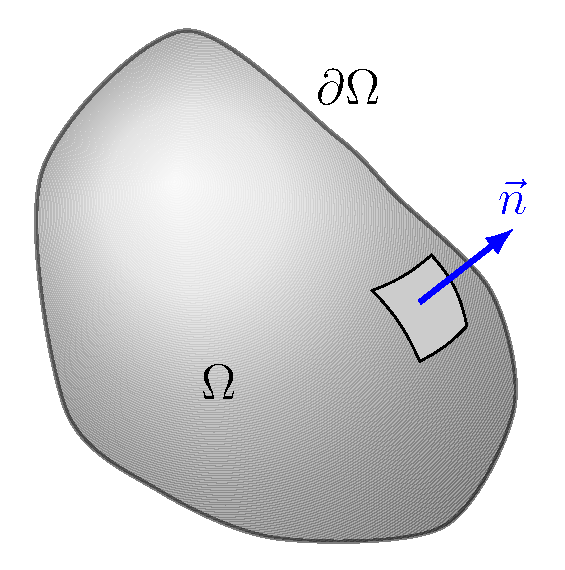
\includegraphics[scale=1]{Imagenes/Funcion_Green_01.pdf}
\caption{Consideremos la ecuación de Poisson dentro de una región $\Omega$ acotada por una superficie $\partial \Omega$}
\label{fig:figura_07_01}
\end{figure}
\end{frame}

\begin{frame}
\frametitle{Ecuación no homogénea}
Esta es la forma no homogénea de la ecuación de Laplace.
\\
\bigskip
\pause
El término no homogéneo, $f (\vb{r})$, podría representar una fuente de calor en un problema de estado estacionario o una distribución de carga (fuente) en un problema electrostático.
\end{frame}

\begin{frame}
\frametitle{Considerando la fuente}
Ahora pensemos en la fuente como una fuente puntual en la que estamos interesados en la respuesta del sistema a esta fuente puntual.
\\
\bigskip
\pause
Si la fuente puntual está ubicada en un punto $\vb{\pderivada{r}}$, entonces la respuesta a la fuente puntual podría sentirse en los puntos $\vb{r}$.
\end{frame}

\begin{frame}
\frametitle{Estableciendo un nombre}
Llamaremos a esta respuesta $G(\vb{r}, \vb{\pderivada{r}})$. \pause La función de respuesta satisfaceria una ecuación de fuente puntual de la forma:
\pause
\begin{align*}
\laplacian G(\vb{r}, \vb{\pderivada{r}}) = \delta (\vb{r} - \vb{\pderivada{r}})
\end{align*}
donde $\delta (\vb{r} - \vb{\pderivada{r}})$ es la función delta de Dirac.
\end{frame}

\begin{frame}
\frametitle{Propiedad de filtro de $\delta (r)$}
Una propiedad clave de esta función generalizada es la propiedad de filtro:
\pause
\begin{align*}
\scaleint{6ex}_{\bs \Omega} \delta (\vb{r} - \vb{\pderivada{r}}) \, f (\vb{r}) \dd{V} = f (\vb{\pderivada{r}})
\end{align*}
\end{frame}

\begin{frame}
\frametitle{Relación entre la función de Green y la solución}
La conexión entre la función de Green y la solución a la ecuación de Poisson se encuentra en la segunda identidad de Green:
\pause
\begin{align*}
\scaleint{6ex}_{\bs \partial \Omega} \bigg[ \phi \, \grad{\psi} - \psi \, \grad{\phi} \bigg] \cdot \vb{n} \dd{S} = \scaleint{6ex}_{\bs \Omega} \bigg[ \phi \, \laplacian{\psi} - \psi \, \laplacian{\phi} \bigg] \dd{V}
\end{align*}
\end{frame}

\begin{frame}
\frametitle{Usando la identidad}
Haciendo que $\phi = u (\vb{r})$ y $\psi = G (\vb{r}, \vb{\pderivada{r}})$, \pause considera que a continuación las integrales de volumen y de superficie, así como la diferenciación usando el operador $\grad$ se realizan usando las $\vb{r}$-coordenadas.
\end{frame}

\begin{frame}
\frametitle{Usando la identidad}
Se tiene que:
\fontsize{12}{12}\selectfont
\begin{eqnarray}
\begin{aligned}[b]
&\scaleint{6ex}_{\bs \partial \Omega} \bigg[ u (\vb{r}) \, \grad{G (\vb{r}, \vb{\pderivada{r}})} - G (\vb{r}, \vb{\pderivada{r}}) \, \grad{u (\vb{r})} \bigg] \cdot \vb{n} \dd{S} = \\[0.5em] \pause
&= \scaleint{6ex}_{\bs \Omega} \bigg[ u (\vb{r}) \, \laplacian{G (\vb{r}, \vb{\pderivada{r}})} - G (\vb{r}, \vb{\pderivada{r}}) \, \laplacian{u (\vb{r})} \bigg] \dd{V} = \\[0.5em] \pause
&= \scaleint{6ex}_{\bs \Omega} \bigg[ u (\vb{r}) \, \delta (\vb{r} - \vb{\pderivada{r}}) - G (\vb{r}, \vb{\pderivada{r}}) \, f (\vb{r}) \bigg] \dd{V} = \\[0.5em] \pause
&= u (\vb{\pderivada{r}}) - \scaleint{6ex}_{\bs \Omega} G (\vb{r}, \vb{\pderivada{r}}) \, f (\vb{r}) \dd{V}
\end{aligned}
\label{eq:ecuacion_07_02}
\end{eqnarray}
\end{frame}

\begin{frame}
\frametitle{Resolviendo la expresión}
Al resolver para $u (\vb{\pderivada{r}})$, se tiene que:
\pause
\begin{eqnarray}
\begin{aligned}[b]
&u (\vb{\pderivada{r}}) = \scaleint{6ex}_{\bs \Omega} G (\vb{r}, \vb{\pderivada{r}}) \, f (\vb{r}) \dd{V} + \\[0.5em] \pause
&+ \scaleint{6ex}_{\bs \partial \Omega} \bigg[ u (\vb{r}) \, \grad{G (\vb{r}, \vb{\pderivada{r}})} - G (\vb{r}, \vb{\pderivada{r}}) \, \grad{u (\vb{r})} \bigg] \cdot \vb{n} \dd{S}
\end{aligned}
\label{eq:ecuacion_07_03}
\end{eqnarray}
\end{frame}

\begin{frame}
\frametitle{Ocupando las condiciones del problema}
Si tanto $u (\vb{r})$ como $G (\vb{r}, \vb{\pderivada{r}})$ satisfacen las condiciones de Dirichlet, $u = 0$ en $\partial \Omega$, \pause entonces la última integral se anula y nos queda:
\begin{align*}
u (\vb{\pderivada{r}}) = \scaleint{6ex}_{\bs \Omega} G (\vb{r}, \vb{\pderivada{r}}) \, f (\vb{r}) \dd{V}
\end{align*}
\end{frame}

\begin{frame}
\frametitle{Casos con simetría}
En algunas aplicaciones se presenta la simetría:
\pause
\begin{align*}
G (\vb{r}, \vb{\pderivada{r}}) = G (\vb{\pderivada{r}}, \vb{r})
\end{align*}
\pause
Por lo que el resultado se puede escribir como:
\pause
\begin{align*}
u (\vb{\pderivada{r}}) = \scaleint{6ex}_{\bs \Omega} G (\vb{r}, \vb{\pderivada{r}}) \, f (\vb{\pderivada{r}}) \dd{\pderivada{V}}
\end{align*}
\end{frame}

\begin{frame}
\frametitle{Resultado importante}
Entonces, si conocemos la función de Green, \pause \textocolor{red}{podemos resolver la ED no homogénea}.
\\
\bigskip
\pause
De hecho, podemos usar la función de Green para resolver problemas de valor límite y valor inicial no homogéneos.
\end{frame}

\section{Funciones de Green para valores iniciales}
\frame[allowframebreaks]{\tableofcontents[currentsection, hideothersubsections]}
\subsection{Planteamiento}

\begin{frame}
\frametitle{Tipo de problemas a resolver}
En esta parte revisaremos la solución de problemas con valores iniciales que involucran ED no homogéneas utilizando las funciones de Green.
\end{frame}

\begin{frame}
\frametitle{Tipo de ED}
Nuestro objetivo es resolver la ED no homogénea:
\pause
\begin{align}
a (t) \, \sderivada{y} (t) + b (t) \, \pderivada{y} (t) + c (t) \, y (t) = f (t)
\label{eq:ecuacion_07_04}
\end{align}
\pause
sujeta a las condiciones iniciales (CI):
\pause
\begin{align*}
y (0) = y_{0} \hspace{1cm} \pderivada{y} (0) = v_{0}
\end{align*}
\end{frame}

\begin{frame}
\frametitle{Reasignado la variable independiente}
Como estamos interesados en problemas de valor inicial, denotaremos la variable independiente como una variable temporal: $t$.
\\
\bigskip
\pause
La ec. (\ref{eq:ecuacion_07_04}) se puede escribir de forma compacta como:
\pause
\begin{align*}
L [y] = f
\end{align*}
\pause
donde $L$ es el operador diferencial:
\begin{align*}
L = a (t) \, \dv[2]{t} + b (t) \, \dv{t} + c (t) 
\end{align*}
\end{frame}

\begin{frame}
\frametitle{Solución al problema}
Cuya solución está dada por:
\pause
\begin{align*}
y = L^{-1} [f]
\end{align*}
\end{frame}

\begin{frame}
\frametitle{El inverso del operador}
El inverso de un operador diferencial es un operador integral, que buscamos escribir en la forma:
\pause
\begin{align*}
y (t) = \scaleint{6ex} G (t, \tau) \, f(\tau) \dd{\tau}
\end{align*}
\pause
La función $G (t, \tau)$ se conoce como el  \textocolor{ao}{kernel} (núcleo) del operador integral y  se denomina \textocolor{carmine}{función de Green}.
\end{frame}

\begin{frame}
\frametitle{Apoyo del curso de EDO1}
Tomando del curso de Ecuaciones Diferenciales I la parte de solución con el \textocolor{armygreen}{método de variación de parámetros}, \pause recordemos que este método es un procedimiento útil para la obtención de una solución particular $y_{p} (x)$ de la EDO lineal (no homogénea) y se basa en el conocimiento de la solución general de la lineal homogénea asociada a dicha EDO lineal.
\end{frame}

\begin{frame}
\frametitle{Seguimos entonces}
Hacemos que:
\pause
\begin{align}
y_{p} (t) = c_{1} (t) \, y_{1} (t) + c_{2} (t) \, y_{2} (t)
\label{eq:ecuacion_07_05}
\end{align}
\end{frame}

\begin{frame}
\frametitle{Sistema por resolver}
Encontramos que tenemos que resolver el sistema de ecuaciones:
\pause
\begin{eqnarray}
\begin{aligned}[b]
\pderivada{c}_{1} (t) \, y_{1} (t) + \pderivada{c}_{2} (t) \, y_{2} (t) &= 0 \\[0.5em] \pause
\pderivada{c}_{1} (t) \, \pderivada{y}_{1} (t) + \pderivada{c}_{2} (t) \, \pderivada{y}_{2} (t) &= \dfrac{f (t)}{q (t)}
\end{aligned}
\label{eq:ecuacion_07_06}
\end{eqnarray}
\end{frame}

\begin{frame}
\frametitle{Resolviendo el sistema}
Este sistema se resuelve fácilmente, para obtener entonces:
\pause
\begin{eqnarray}
\begin{aligned}[b]
\pderivada{c}_{1} (t) &= - \dfrac{f (t) \, y_{2} (t)}{a (t) \big[ y_{1} (t) \, \pderivada{y}_{2} (t)  - \pderivada{y}_{1} (t) \, y_{2} (t) \big]} \\[0.5em] \pause
\pderivada{c}_{2} (t) &= \dfrac{f (t) \, y_{1} (t)}{a (t) \big[ y_{1} (t) \, \pderivada{y}_{2} (t)  - \pderivada{y}_{1} (t) \, y_{2} (t) \big]}
\end{aligned}
\label{eq:ecuacion_07_07}
\end{eqnarray}
\end{frame}

\begin{frame}
\frametitle{Usando el Wronskiano}
Notemos que el denominador en estas expresiones involucra el Wronskiano de las soluciones al problema homogéneo, el cual viene dado por el determinante:
\pause
\begin{align*}
W (y_{1}, y_{2}) (t) = \mqty|
y_{1} (t) & y_{2} (t) \\
\pderivada{y}_{1} (t) & \pderivada{y}_{2} (t) |
\end{align*}
\end{frame}

\begin{frame}
\frametitle{Soluciones linealmente independientes}
Cuando $y_{1} (t)$ y $y_{2} (t)$ son linealmente independientes, \pause entonces el Wronskiano no es cero y tenemos garantizada una solución para el sistema anterior.
\end{frame}

\begin{frame}
\frametitle{Integrando el sistema}
Entonces, después de una integración, encontramos los parámetros como:
\pause
\begin{eqnarray}
\begin{aligned}
c_{1} (t) &= - \scaleint{6ex}_{\bs t_{0}}^{t} \dfrac{f (\tau) \, y_{2} (\tau)}{a (\tau) \, W (\tau)} \dd{\tau} \\[0.5em] \pause
c_{2} (t) &= \scaleint{6ex}_{\bs t_{1}}^{t} \dfrac{f (\tau) \, y_{1} (\tau)}{a (\tau) \, W (\tau)} \dd{\tau}
\end{aligned}
\label{eq:ecuacion_07_08}
\end{eqnarray}
donde $t_{0}$ y $t_{1}$ son constantes arbitrarias que se determinarán a partir de las condiciones iniciales.
\end{frame}

\begin{frame}
\frametitle{Solución particular}
Por lo tanto, la solución particular de la ec. (\ref{eq:ecuacion_07_04}) se puede escribir como:
\pause
\begin{eqnarray}
\begin{aligned}
y_{p} (t) &= y_{2} (t) \scaleint{6ex}_{\bs t_{1}}^{t} \dfrac{f (\tau) \, y_{1} (\tau)}{a (\tau) \, W (\tau)} \dd{\tau} + \\[0.5em] 
&- y_{1} (t) \scaleint{6ex}_{\bs t_{0}}^{t} \dfrac{f (\tau) \, y_{2} (\tau)}{a (\tau) \, W (\tau)} \dd{\tau}
\end{aligned}
\label{eq:ecuacion_07_09}
\end{eqnarray}
\end{frame}

\begin{frame}
\frametitle{Obteniendo las soluciones}
Comenzamos con la solución particular de la ec. (\ref{eq:ecuacion_07_09}) de la ED no homogénea (\ref{eq:ecuacion_07_04}).
\end{frame}

\begin{frame}
\frametitle{Obteniendo las soluciones}Esta se puede combinar con la solución general del problema homogéneo para dar la solución general de la ED no homogénea:
\begin{eqnarray}
\begin{aligned}
y_{p} (t) &= c_{1} y_{1} (t) + c_{2} y_{2} (t) +  y_{2} (t) \scaleint{6ex}_{\bs t_{1}}^{t} \dfrac{f (\tau) \, y_{1} (\tau)}{a (\tau) \, W (\tau)} \dd{\tau} + \\[0.5em] 
&- y_{1} (t) \scaleint{6ex}_{\bs t_{0}}^{t} \dfrac{f (\tau) \, y_{2} (\tau)}{a (\tau) \, W (\tau)} \dd{\tau}
\label{eq:ecuacion_07_10}
\end{aligned}
\end{eqnarray}
\end{frame}

\begin{frame}
\frametitle{Elección oportuna}
Sin embargo, se puede encontrar una elección adecuada de $t_{0}$ y $t_{1}$ para que no necesitemos escribir explícitamente la solución al problema homogéneo, $c_{1} y_{1} (t) + c_{2} y_{2} (t)$. 
\\
\bigskip
\pause
No obstante, configurar la solución de esta forma nos permitirá usar $t_{0}$ y $t_{1}$ para determinar soluciones particulares que satisfagan ciertas condiciones homogéneas.
\end{frame}

\begin{frame}
\frametitle{Usando la función de Green}
En particular, mostraremos que la ec. (\ref{eq:ecuacion_07_10}) se puede escribir en la forma:
\pause
\begin{align}
y_{p} (t) = c_{1} y_{1} (t) + c_{2} y_{2} (t) +  y_{2} (t) \scaleint{6ex}_{\bs 0}^{t} G (t,\tau) \, f (\tau) \dd{\tau}
\label{eq:ecuacion_07_11}
\end{align}
donde la función $G (t, \tau)$ será identificada como la función de Green.
\end{frame}

\begin{frame}
\frametitle{Tipos de problemas}
El objetivo es entonces desarrollar la técnica de la función de Green para resolver el problema de valor inicial:
\pause
\begin{eqnarray}
\begin{aligned}
a (t) \, \sderivada{y} (t) + b (t) \, &\pderivada{y} (t) + c (t) y(t) = f (t) \\[0.5em]
y (0) = y_{0}, \hspace{0.7cm} &\pderivada{y} (0) = v_{0}
\end{aligned}
\label{eq:ecuacion_07_12}
\end{eqnarray}
\end{frame}

\begin{frame}
\frametitle{Revisando el tipo de problemas}
Primero observamos que podemos resolver este problema de valores iniciales resolviendo dos problemas de valores iniciales separados.
\\
\bigskip
\pause
Suponemos que la solución del problema homogéneo satisface las condiciones iniciales originales:
\pause
\begin{eqnarray}
\begin{aligned}
a (t) \, \sderivada{y}_{h} (t) + b (t) \, &\pderivada{y}_{h} (t) + c (t) y_{h} (t) = f (t) \\
y_{h} (0) = y_{0}, \hspace{0.7cm} &\pderivada{y}_{h} (0) = v_{0}
\end{aligned}
\label{eq:ecuacion_07_13}
\end{eqnarray}
\end{frame}

\begin{frame}
\frametitle{Solución particular}
Entonces asumimos que la solución particular satisface el problema:
\pause
\begin{eqnarray}
\begin{aligned}
a (t) \, \sderivada{y}_{p} (t) + b (t) \, &\pderivada{y}_{p} (t) + c (t) y_{h} (t) = f (t) \\[0.5em]
y_{p} (0) = y_{0}, \hspace{0.2cm} &\pderivada{y}_{p} (0) = v_{0}
\end{aligned}
\label{eq:ecuacion_07_14}
\end{eqnarray}
\end{frame}

\begin{frame}
\frametitle{Aprovechando la linealidad}
Dado que la ED es lineal, se sabe que:
\pause
\begin{align*}
y (t) = y_{h} (t) + y_{p} (t)
\end{align*}
es una solución a la ecuación no homogénea.
\end{frame}

\begin{frame}
\frametitle{Solución que satisface las CI}
También, esta solución satisface las condiciones iniciales:
\pause
\begin{align*}
y (0) &= y_{h} (0) + y_{p} (0) = y_{0} + 0 = y_{0} \\[0.5em]
\pderivada{y} (0) &= \pderivada{y}_{h} (0) + \pderivada{y}_{p} (0) = v_{0} + 0 = v_{0}
\end{align*}
\end{frame}

\begin{frame}
\frametitle{Solución que cumpla las CI}
Por lo tanto, solo debemos centrarnos en encontrar una solución particular que satisfaga las condiciones iniciales homogéneas.
\\
\bigskip
\pause
Esto se hará encontrando valores para $t_{0}$ y $t_{1}$ en la ec. (\ref{eq:ecuacion_07_09}) que satisfagan las condiciones iniciales homogéneas: $y_{p} (0) = 0$ y $\pderivada{y}_{p} (0) = 0$
\end{frame}

\begin{frame}
\frametitle{Considerando un valor}
Primero, consideramos $y_{p} (0) = 0$. \pause Tenemos que:
\pause
\begin{eqnarray}
\begin{aligned}
y_{p} (0) &= y_{2} (0) \scaleint{6ex}_{\bs t_{1}}^{0} \dfrac{f (\tau) \, y_{1} (\tau)}{a (\tau) \, W (\tau)} \dd{\tau} + \\[0.5em]
&- y_{1} (0) \scaleint{6ex}_{\bs t_{0}}^{t} \dfrac{f (\tau) \, y_{2} (\tau)}{a (\tau) \, W (\tau)} \dd{\tau}
\end{aligned}
\label{eq:ecuacion_07_15}
\end{eqnarray}
Aquí, $y_{1} (t)$ y $y_{2} (t)$ se toman como cualquier solución de la ED homogénea.
\end{frame}
\begin{frame}
\frametitle{Suponiendo un caso}
Supongamos que $y_{1} (0) = 0$ y $y_{2} (0) \neq 0$. \pause Entonces, tenemos:
\pause
\begin{align}
y_{p} (0) = y_{2} (0) \scaleint{6ex}_{\bs t_{1}}^{0} \dfrac{f (\tau) \, y_{1} (\tau)}{a (\tau) \, W (\tau)} \dd{\tau}
\label{eq:ecuacion_07_16}
\end{align}
\pause
Podemos forzar que $y_{p} (0) = 0$ si hacemos que $t_{1} = 0$.
\end{frame}
\begin{frame}
\frametitle{Considerando otro valor}
Ahora, consideramos $\pderivada{y}_{p} (0) = 0$. \pause Primero derivamos la solución y encontramos que:
\pause
\begin{eqnarray}
\begin{aligned}
\pderivada{y}_{p} (t) &= \pderivada{y}_{2} (t) \scaleint{6ex}_{\bs 0}^{t} \dfrac{f (\tau) \, y_{1} (\tau)}{a (\tau) \, W (\tau)} \dd{\tau} + \\[0.5em]
&- \pderivada{y}_{1} (t) \scaleint{6ex}_{\bs t_{0}}^{t} \dfrac{f (\tau) \, y_{2} (\tau)}{a (\tau) \, W (\tau)} \dd{\tau}
\end{aligned}
\label{eq:ecuacion_07_17}
\end{eqnarray}
ya que las contribuciones al diferenciar las integrales se cancelarán.
\end{frame}
\begin{frame}
\frametitle{Evaluando el resultado}
Evaluando este resultado en $t = 0$, tenemos:
\pause
\begin{align}
\pderivada{y}_{p} (0) = - \pderivada{y}_{1} (0) \scaleint{6ex}_{\bs t_{0}}^{0} \dfrac{f (\tau) \, y_{2} (\tau)}{a (\tau) \, W (\tau)} \dd{\tau}
\label{eq:ecuacion_07_18}
\end{align}
Suponiendo que $\pderivada{y}_{p} (0) \neq 0$, podemos hacer que $t_{0} = 0$.
\end{frame}

\begin{frame}
\frametitle{Resultado obtenido}
Entonces, hemos encontrado que:
\pause
\begin{eqnarray}
\begin{aligned}[b]
y_{p} (x) &= y_{2} (t) \scaleint{6ex}_{\bs 0}^{t} \dfrac{f (\tau) \, y_{1} (\tau)}{a (\tau) \, W (\tau)} \dd{\tau} + \\[0.5em]
&- y_{1} (t) \scaleint{6ex}_{\bs t_{0}}^{t} \dfrac{f (\tau) \, y_{2} (\tau)}{a (\tau) \, W (\tau)} \dd{\tau} = \\[0.5em] \pause
&= \scaleint{6ex}_{\bs 0}^{t} \bigg[ \dfrac{y_{1} (\tau) \, y_{2} (t) - y_{1} (t) \, y_{2} (\tau)}{a (\tau) \, W (\tau)} \bigg] \, f (\tau) \dd{\tau}
\end{aligned}
\label{eq:ecuacion_07_19}
\end{eqnarray}
\end{frame}

\begin{frame}
\frametitle{Expresión conocida}
Este resultado está en la forma correcta y podemos identificar el valor temporal o inicial: \textocolor{ao}{la función de Green}. \pause Entonces, la solución particular se da como:
\pause
\begin{align}
y_{p} (t) = \scaleint{6ex}_{\bs 0}^{t} G (t, \tau) \, f (\tau) \dd{\tau}
\label{eq:ecuacion_07_20}
\end{align}
\pause
donde la condición inicial de la función de Green está definida como:
\begin{align*}
G (t, \tau) = \dfrac{y_{1} (\tau) \, y_{2} (t) - y_{1} (t) \, y_{2} (\tau)}{a (\tau) \, W (\tau)}
\end{align*}
\end{frame}

\begin{frame}[plain]
\begin{tcolorbox}[title={\centering Solución para problema de valores iniciales con la función de Green}]
La solución al problema de valores iniciales:
\begin{align*}
a (t) \, \sderivada{y} (t) + b (t) &\pderivada{y} (t) + c (t) \, y (t) = f (t) \\[0.5em]
y (0) = y_{0}, \hspace{0.2cm} &\pderivada{y} (0) = v_{0}
\end{align*}
\pause
es de la forma:
\begin{align}
y (t) = y_{h} (t) + \scaleint{6ex}_{\bs 0}^{t} G (t, \tau) \, f (t) \dd{\tau}
\label{eq:ecuacion_07_21}
\end{align}
\end{tcolorbox}
\end{frame}

\begin{frame}[plain]
\begin{tcolorbox}[title={\centering Solución para problema de valores iniciales con la función de Green}]
Donde:
\begin{align}
G (t, \tau) = \dfrac{y_{1} (\tau) \, y_{2} (t) - y_{1} (t) \, y_{2} (\tau)}{a (\tau) \, W (\tau)}
\label{eq:ecuacion_07_22}
\end{align}
es la función de Green, \pause $y_{1}$, $y_{2}$, $y_{h}$ son soluciones de la ecuación homogénea que satisfacen:
\begin{align*}
&y_{1} (0) {=} 0, \hspace{0.2cm} y_{2} (0) {\neq} 0, \hspace{0.2cm} \pderivada{y}_{1} (0) {\neq} 0, \\[0.5em]
&\pderivada{y}_{2} (0) {=} 0, \hspace{0.2cm} y_{h} (0) {=} y_{0}, \hspace{0.2cm} \pderivada{y}_{h} (0) {=} v_{0}
\end{align*}
\end{tcolorbox}
\end{frame}

\subsection{Ejercicio}

\begin{frame}
\frametitle{Ejemplo a resolver}
Resolvamos el problema del oscilador forzado:
\pause
\begin{align*}
\sderivada{x} + x = 2 \, \cos t, \hspace{0.5cm} x (0) = 4, \hspace{0.2cm} \pderivada{x} (0) = 0
\end{align*}
\end{frame}

\begin{frame}
\frametitle{Primera solución}
Primero resolvemos el problema homogéneo con las condiciones iniciales no homogéneas:
\pause
\begin{align*}
\sderivada{x}_{h} + x_{h} = 0, \hspace{0.5cm} x_{h} (0) = 4, \hspace{0.2cm} \pderivada{x}_{h} (0) = 0
\end{align*}
\pause
Cuya solución se obtiene fácilmente: $x_{h} (t) = 4 \, \cos t$, que se presenta en la figura (\ref{fig:figura_01}).
\end{frame}

\begin{frame}
\frametitle{Gráfica de la solución}
\begin{figure}[H]
    \centering
    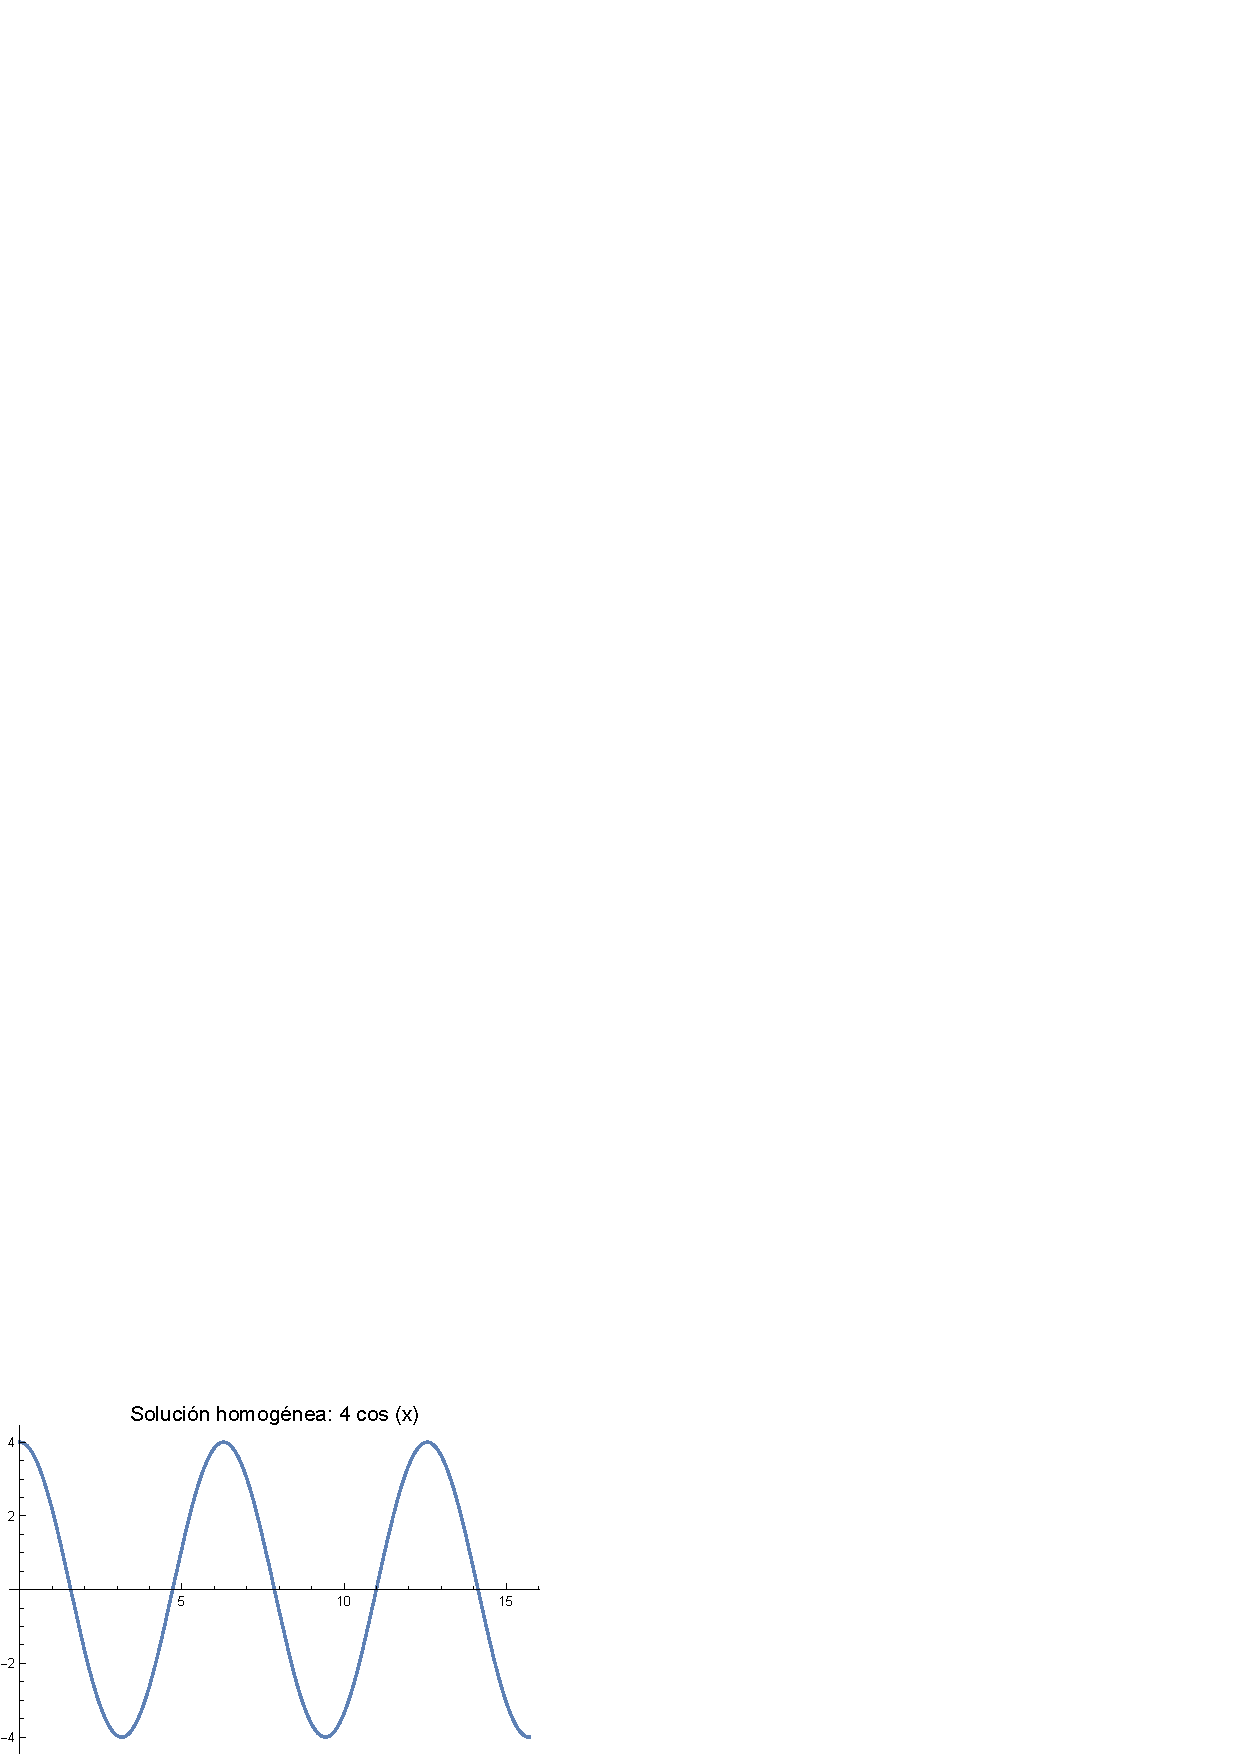
\includegraphics[scale=0.7]{Imagenes/Plot_Oscilador_Forzado_Green_01.pdf}
    \caption{Primer resultado}
    \label{fig:figura_01}
\end{figure} 
\end{frame}
\begin{frame}
\frametitle{Siguiente paso en la solución}
A continuación, construimos la función de Green.
\\
\bigskip
\pause
Necesitamos dos soluciones linealmente independientes, $y_{1} (x)$, $y_{2} (x)$, para la ED homogénea que satisfaga diferentes condiciones homogéneas, $y_{1} (0) = 0$ y $\pderivada{y}_{2} (0) = 0$. \pause Las soluciones más simples son $y_{1} (t) = \sen t$ y $y_{2} (t) = \cos t$.
\end{frame}

\begin{frame}
\frametitle{Recuperando el Wronskiano}
El Wronskiano para este ejemplo es:
\pause
\begin{eqnarray*}
\begin{aligned}
W (t) &= y_{1} (t) \, \pderivada{y}_{2} (t) - \pderivada{y}_{1} (t) \, y_{2} (t) = \\[0.5em] \pause
&=  - \sin^{2} (t) - \cos^{2} (t) = \\[0.5em] \pause
&= \pause - 1 
\end{aligned}
\end{eqnarray*}
\end{frame}

\begin{frame}
\frametitle{La función de Green}
Dado que en este ejercicio $a (t) = 1$, es posible calcular la función de Green:
\pause
\begin{eqnarray}
\begin{aligned}[b]
G (t, \tau) &= G (t, \tau) = \dfrac{y_{1} (\tau) \, y_{2} (t) - y_{1} (t) \, y_{2} (\tau)}{a (\tau) \, W (\tau)} = \\[0.5em] \pause
&= \sin t \, \cos \tau - \sin \tau \, \cos t = \\[0.5em] \pause
&= \sin (t - \tau)
\end{aligned}
\label{eq:ecuacion_07_23}
\end{eqnarray}
\end{frame}

\begin{frame}
\frametitle{Consideranción importante}
Tomemos en cuenta que la función de Green depende de $t - \tau$.
\\
\bigskip
\pause
Si bien esto es útil en algunos contextos, usaremos la forma expandida al realizar la integración.
\end{frame}

\begin{frame}
\frametitle{La solución particular}
Ahora podemos determinar la solución particular de la ED no homogénea. \pause Tenemos que:
\pause
\begin{eqnarray*}
\begin{aligned}
x_{p} (t) &= \scaleint{6ex}_{\bs 0}^{t} G (t, \tau) \, f (\tau) \dd{\tau} = \\[0.5em]  \pause
&= \scaleint{6ex}_{\bs 0}^{t} (\sin t \, \cos \tau - \sin \tau \, \cos t) (2 \, \cos \tau) \dd{\tau} = \\[0.5em] \pause
&= 2 \sin t \, \scaleint{6ex}_{\bs 0}^{t} \cos^{2} \tau \dd{\tau} - 2 \cos t \, \scaleint{6ex}_{\bs 0}^{t} \sin \tau \, \cos \tau \dd{\tau} =
\end{aligned}
\end{eqnarray*}
\end{frame}

\begin{frame}
\frametitle{La solución particular}
\begin{eqnarray}
\begin{aligned}    
&= 2 \sin t \, \bigg[ \dfrac{\tau}{2} + \dfrac{1}{2} \, \sin 2 \tau \bigg] \eval_{0}^{t} - 2 \cos t \, \bigg[ \dfrac{1}{2} \, \sin^{2} \tau \bigg] \eval_{0}^{t} = \\[0.5em] \pause
&= t \, \sin t
\end{aligned}
\label{eq:ecuacion_07_24}
\end{eqnarray}
En la figura (\ref{fig:figura_02}) se muestra la solución al caso no homogéneo.
\end{frame}

\begin{frame}
\frametitle{Gráfica del segundo resultado}
\begin{figure}[H]
    \centering
    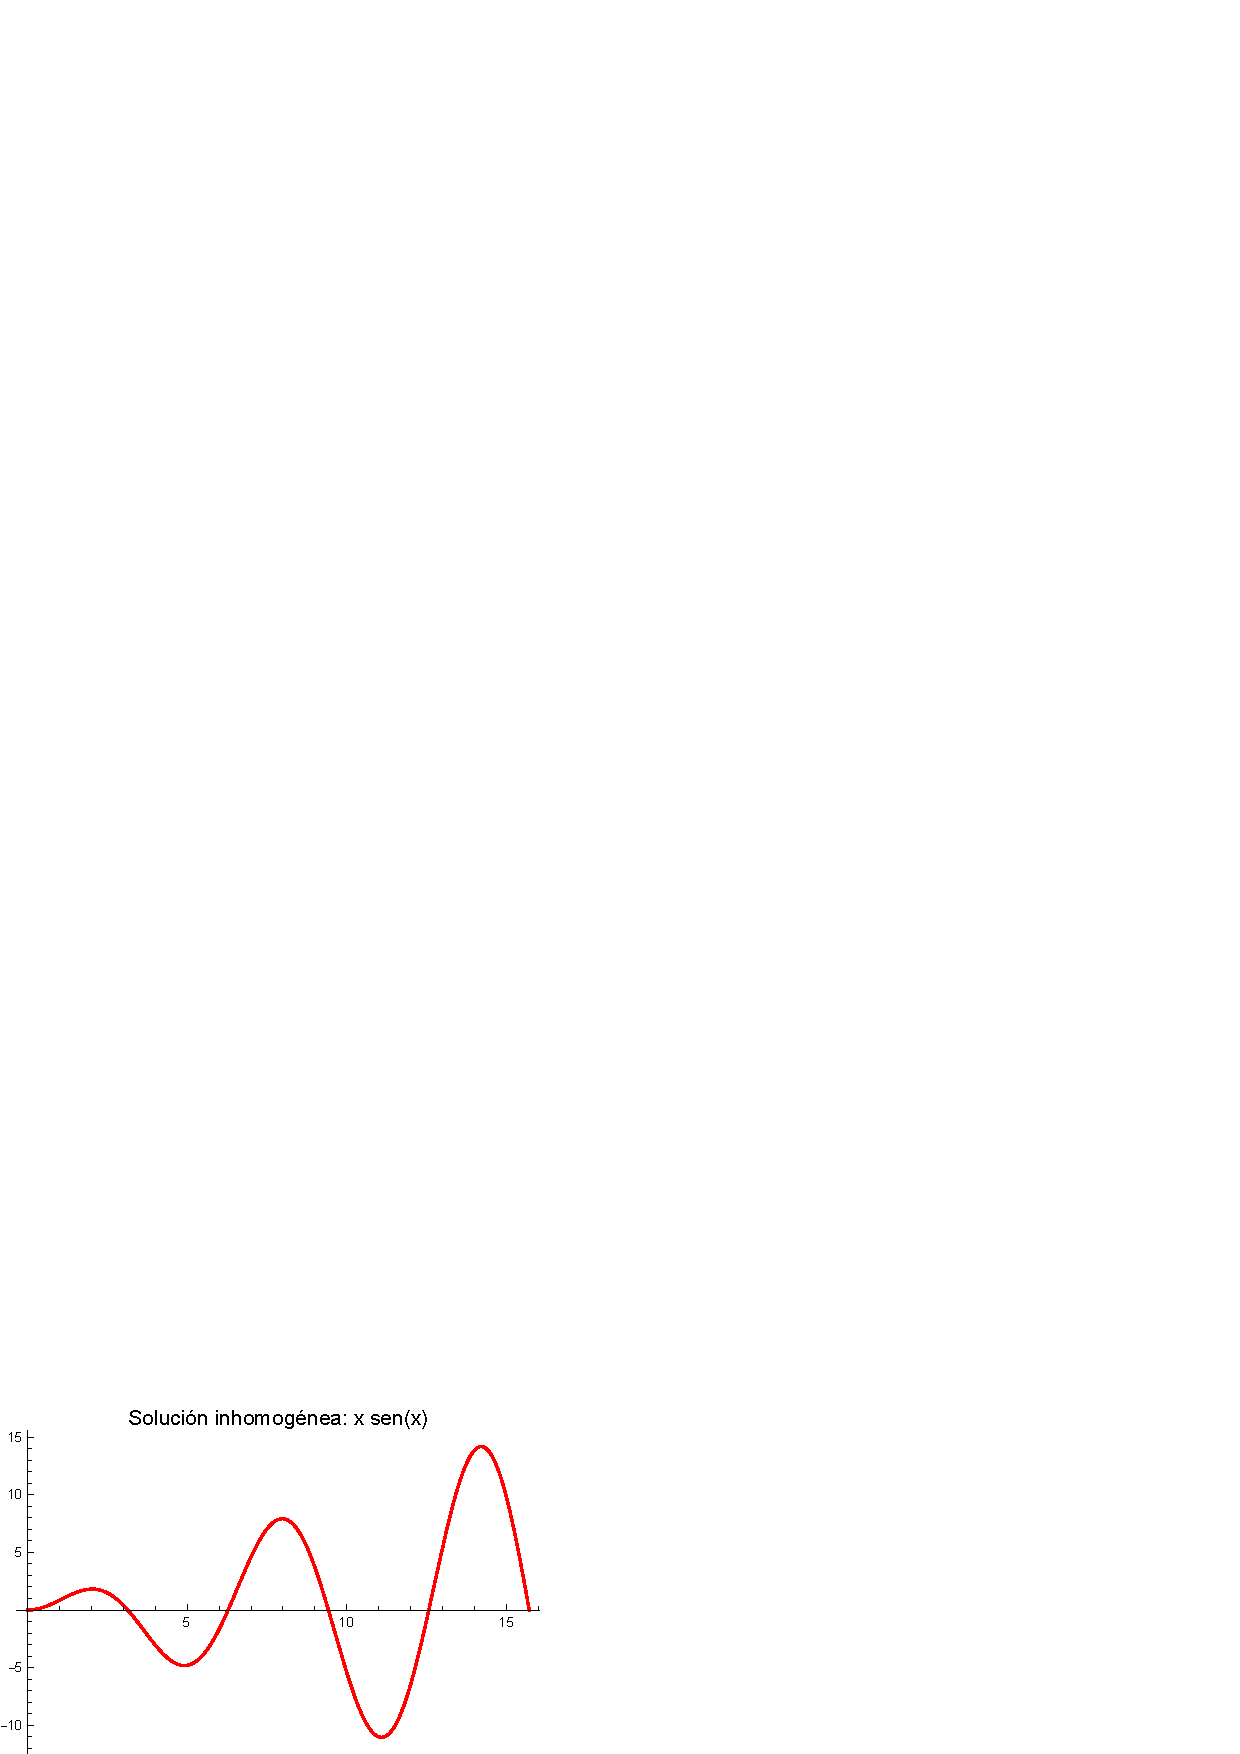
\includegraphics[scale=0.7]{Imagenes/Plot_Oscilador_Forzado_Green_02.pdf}
    \caption{Solución la ED en el caso no homogéneo.}
    \label{fig:figura_02}
\end{figure}
\end{frame}

\begin{frame}
\frametitle{Soluciones a la ED}
\begin{figure}[H]
    \centering
    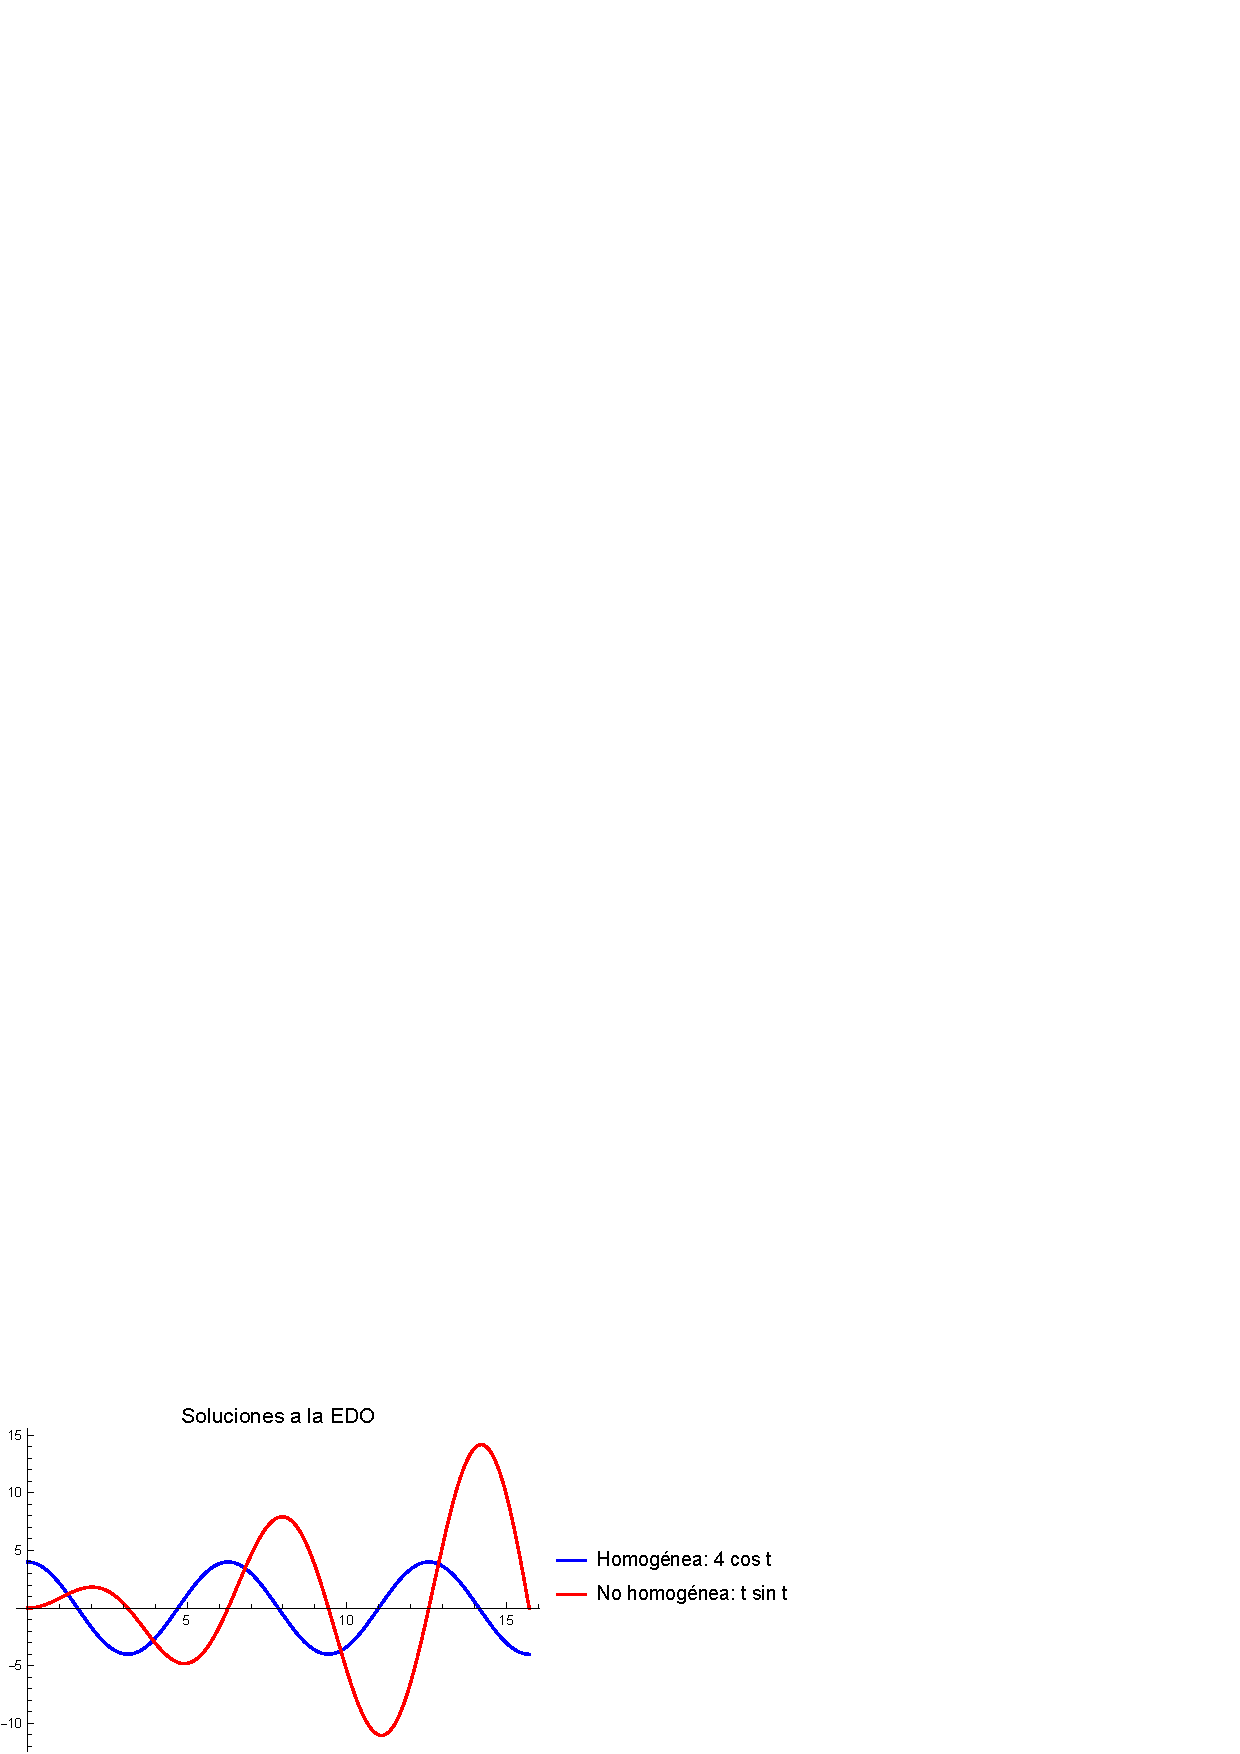
\includegraphics[scale=0.6]{Imagenes/Plot_Oscilador_Forzado_Green_03.pdf}
    \caption{Soluciones a la ED en el caso homogéneo y no homogéneo.}
    \label{fig:figura_03}
\end{figure}
\end{frame}

\begin{frame}
\frametitle{Solución completa}
Por lo tanto, la solución al problema no homogéneo, es la suma es la solución del problema homogéneo y esta solución particular:
\pause
\begin{align*}
x (t) = 4 \, \cos t + t \, \sin t
\end{align*}
La gráfica de la solución se muestra en la figura (\ref{fig:figura_04}):
\end{frame}

\begin{frame}
\frametitle{Solución completa a la ED inhomogénea}
\begin{figure}[H]
    \centering
    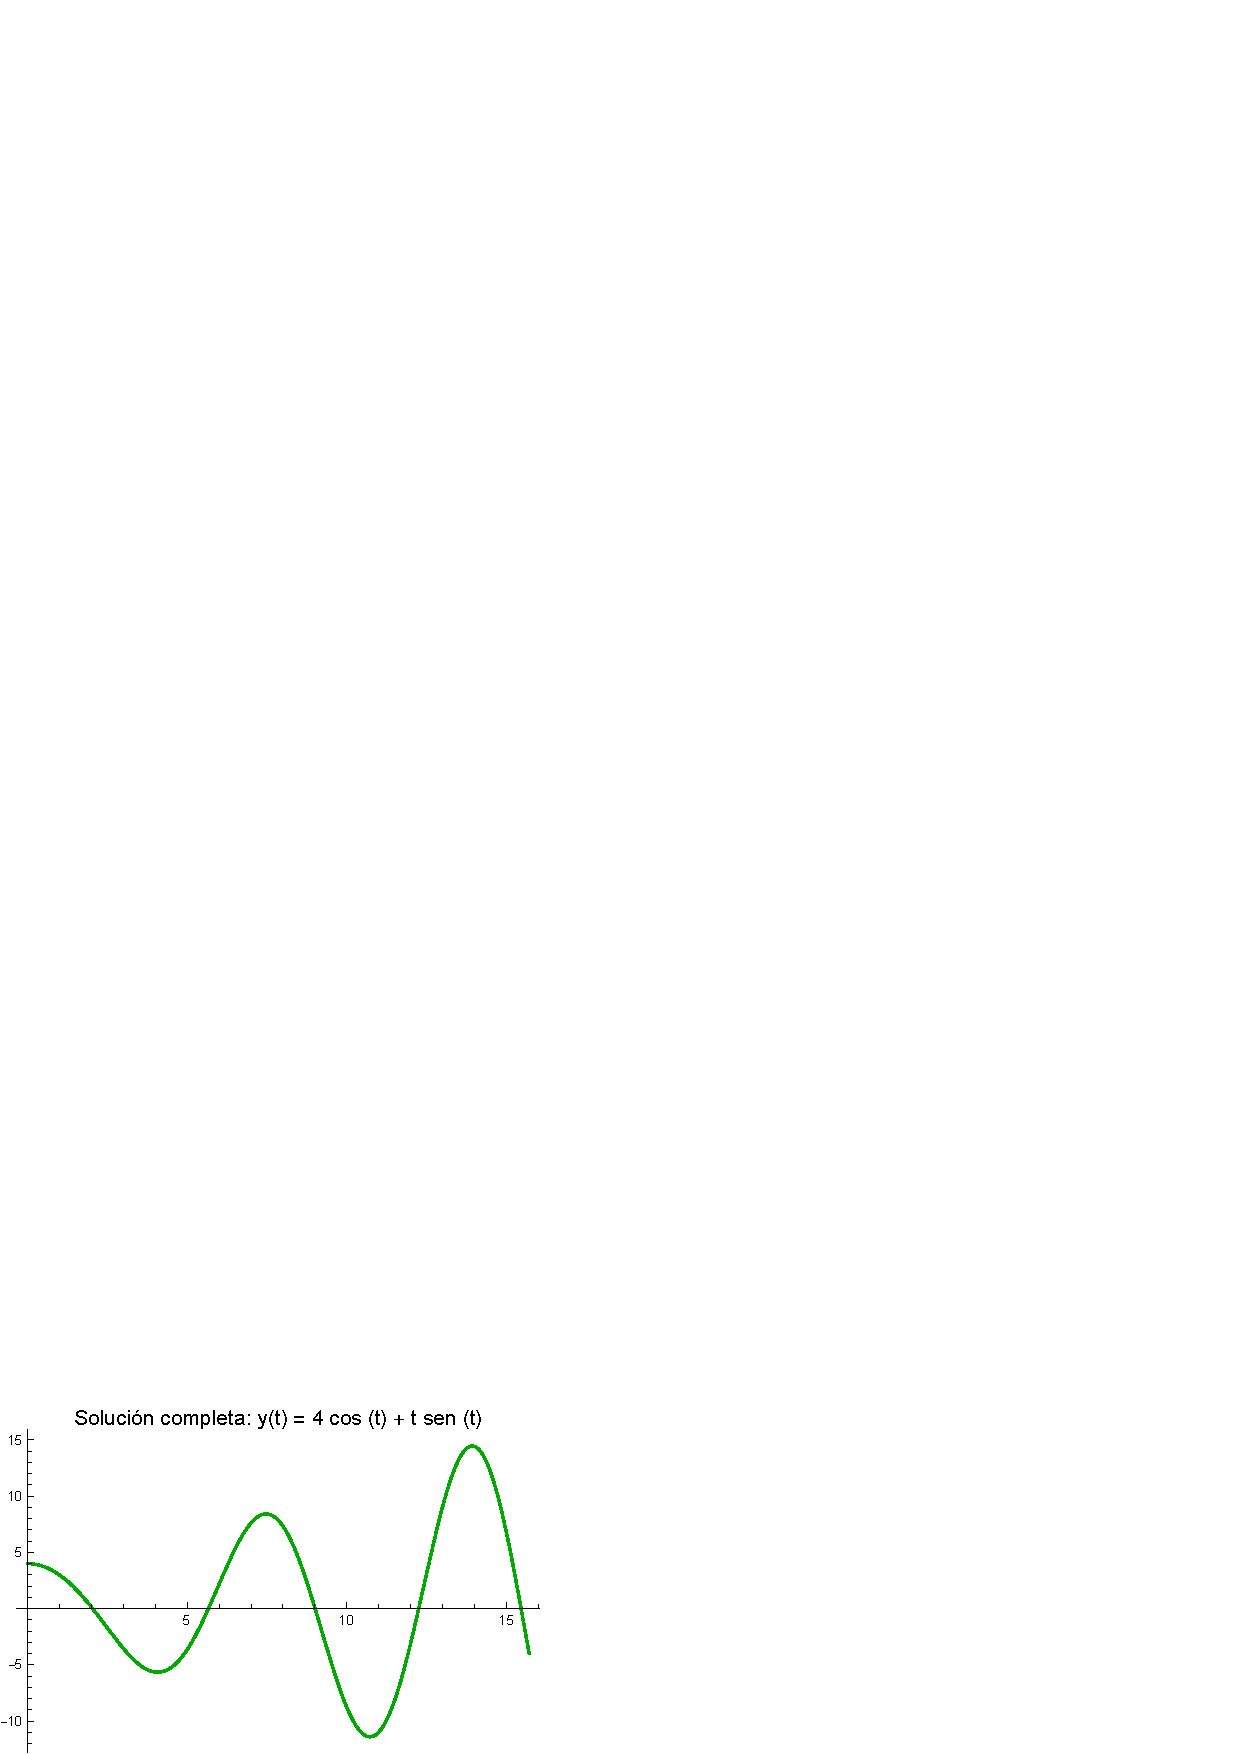
\includegraphics[scale=0.7]{Imagenes/Plot_Oscilador_Forzado_Green_04.pdf}
    \caption{Solución completa a la EDO no homogénea.}
    \label{fig:figura_04}
\end{figure}
\end{frame}


\section{Valores de frontera y funciones de Green.}
\frame{\tableofcontents[currentsection, hideothersubsections]}
\subsection{El problema de estudio}

\begin{frame}
\frametitle{Lo que trabajaremos}
En esta parte extenderemos este método a la solución de problemas con condiciones de frontera no homogéneos usando una función de Green.
\end{frame}

\begin{frame}
\frametitle{Lo que trabajaremos}
Recordemos que el objetivo es resolver la ED no homogénea:
\pause
\begin{align*}
L [y] = f, \hspace{0.6cm} a \leq x \leq b
\end{align*}
donde $L$ es un operador diferencial y $y (x)$ satisface las condiciones de frontera en $x = a$ y $x = b$.
\end{frame}

\begin{frame}
\frametitle{Solución al problema}
La solución viene dada formalmente por:
\pause
\begin{align*}
y = L^{-1} [y]
\end{align*}
\pause
El \textocolor{carmine}{inverso de un operador diferencial es un operador integral}, que buscamos escribir de la forma:
\pause
\begin{align*}
y (x) = \scaleint{6ex}_{a}^{b} G (x, \xi) \, f (\xi) \dd{\xi} 
\end{align*}
La función $G (x, \xi)$ se conoce como el \textocolor{armygreen}{kernel} (núcleo) del operador integral y se le llama \textocolor{cobalt}{función de Green}.
\end{frame}

\begin{frame}
\frametitle{Tipo particular de ED}
Consideraremos problemas CDF de la forma de \textocolor{darkviolet}{Sturm-Liouville}:
\pause
\begin{align}
\dv{x} \bigg[ p (x) \, \dv{y (x)}{x} \bigg] + q (x) \, y (x) = f (x), \hspace{0.6cm} a < x < b
\label{eq:ecuacion_07_25}
\end{align}
con valores fijos de $y (x)$ en la frontera, $y (a) = 0$ y $y (b) = 0$. \pause Sin embargo, la teoría general funciona para otras formas de condiciones de frontera homogéneas.
\end{frame}

\begin{frame}
\frametitle{Solución a la ED}
Buscamos la función de Green resolviendo primero la ED no homogénea usando el \textocolor{byzantine}{método de variación de parámetros}.
\\
\bigskip
\pause
Suponemos una solución particular de la forma:
\pause
\begin{align*}
y_{p} (x) = c_{1} (x) \, y_{1} (x) + c_{2} (x) \, y_{2} (x)
\end{align*}
que se forma a partir de dos soluciones linealmente independientes del problema homogéneo, $y_{i} (x), i = 1, 2$.
\end{frame}

\begin{frame}
\frametitle{Coeficientes que satisfacen el sistema}
Habíamos encontrado que las funciones de los coeficientes satisfacen las ecuaciones:
\pause
\begin{align}
\begin{aligned}[b]
\pderivada{c}_{1} (t) \, y_{1} (t) + \pderivada{c}_{2} (t) \, y_{2} (t) &= 0 \\[0.5em]
\pderivada{c}_{2} (t) \, \pderivada{y}_{1} (t) + \pderivada{c}_{2} (t) \, \pderivada{y}_{2} (t) &= \dfrac{f (t)}{q (t)}
\end{aligned}
\label{eq:ecuacion_07_26}
\end{align}
\end{frame}

\begin{frame}
\frametitle{Resolviendo el sistema}
Resolviendo este sistema, se obtiene:
\pause
\begin{align*}
\pderivada{c}_{1} (x) &= - \dfrac{f \, y_{2}}{p \, W (y_{1}, y_{2})} \\[0.5em]
\pderivada{c}_{2} (x) &= \dfrac{f \, y_{1}}{p \, W (y_{1}, y_{2})}
\end{align*}
donde $W (y_{1}, y_{2}) = y_{1} \, \pderivada{y}_{2} - \pderivada{y}_{1} \, y_{2}$ es el Wronskiano.
\end{frame}

\begin{frame}
\frametitle{Integrando el resultado}
Integrando las expresiones para sustituirlas de regreso en la solución particular, se encuentra que:
\pause
\begin{align*}
y (x) = y_{2} (x) \scaleint{6ex}_{\bs x_{1}}^{x} \dfrac{f (\xi) \, y_{1} (\xi)}{p (\xi) \, W (\xi)} \dd{\xi} - y_{1} (x) \scaleint{6ex}_{\bs x_{0}}^{x} \dfrac{f (\xi) \, y_{2} (\xi)}{p (\xi) \, W (\xi)} \dd{\xi}
\end{align*}
donde $x_{0}$ y $x_{1}$ se determinarán utilizando las condiciones de frontera.
\end{frame}

\begin{frame}
\frametitle{Valores en particular}
En particular, buscaremos $x_{0}$ y $x_{1}$ para que la solución al problema de valores en la frontera pueda escribirse como una integral simple que involucre una función de Green.
\end{frame}

\begin{frame}
\frametitle{Recuperando la solución}
Notemos que podemos absorber la solución del problema homogéneo, $y_{h} (x)$, en las integrales con una elección apropiada de límites en las integrales.
\\
\bigskip
\pause
Ahora buscamos satisfacer las condiciones $y (a) = 0$ y $y (b) = 0$.
\end{frame}

\begin{frame}
\frametitle{Usando las soluciones}
Primero usamos soluciones de la ED homogénea que satisfacen $y_{1} (a) = 0$, $y_{2} (b) = 0$ y $y_{1} (b) \neq 0$, $y_{2} (a) \neq 0$.
\end{frame}

\begin{frame}
\frametitle{Usando las soluciones}
Evaluando $y (x)$ en $x = 0$, tenemos que:
\pause
\begin{eqnarray}
\begin{aligned}[b]
y (a) &= y_{2} (a) \scaleint{6ex}_{\bs x_{1}}^{a} \dfrac{f (\xi) \, y_{1} (\xi)}{p (\xi) \, W (\xi)} \dd{\xi} + \\[0.5em] 
&- y_{1} (a) \scaleint{6ex}_{\bs x_{0}}^{a} \dfrac{f (\xi) \, y_{2} (\xi)}{p (\xi) \, W (\xi)} \dd{\xi} = \\[0.5em] \pause
&= y_{2} (a) \scaleint{6ex}_{\bs x_{1}}^{a} \dfrac{f (\xi) \, y_{1} (\xi)}{p (\xi) \, W (\xi)} \dd{\xi}
\end{aligned}
\label{eq:ecuacion_07_27}
\end{eqnarray}
\end{frame}

\begin{frame}
\frametitle{Eligiendo las condiciones}
Podemos satisfacer la condición en $x = a$ si escogemos $x_{1} = a$. \pause De manera similar, en $x = b$, encontramos que:
\pause
\begin{eqnarray}
\begin{aligned}[b]
y (b) &= y_{2} (b) \scaleint{6ex}_{\bs x_{1}}^{b} \dfrac{f (\xi) \, y_{1} (\xi)}{p (\xi) \, W (\xi)} \dd{\xi} + \\[0.5em]
&- y_{1} (b) \scaleint{6ex}_{\bs x_{0}}^{b} \dfrac{f (\xi) \, y_{2} (\xi)}{p (\xi) \, W (\xi)} \dd{\xi} = \\[0.5em] \pause
&= - y_{1} (b) \scaleint{6ex}_{\bs x_{0}}^{b} \dfrac{f (\xi) \, y_{2} (\xi)}{p (\xi) \, W (\xi)} \dd{\xi}
\end{aligned}
\label{eq:ecuacion_07_28}
\end{eqnarray}
\end{frame}

\begin{frame}
\frametitle{Valor de la condición}
Esta expresión se anula para $x_{0} = b$.
\\
\bigskip
\pause
Así, hemos encontrado que la solución es de la forma:
\pause
\begin{align}
\begin{aligned}[b]
y (x) &= y_{2} (x) \scaleint{6ex}_{\bs a}^{x} \dfrac{f (\xi) \, y_{1} (\xi)}{p (\xi) \, W (\xi)} \dd{\xi} + \\[0.5em]
&- y_{1} (x) \scaleint{6ex}_{\bs b}^{x} \dfrac{f (\xi) \, y_{2} (\xi)}{p (\xi) \, W (\xi)} \dd{\xi}
\end{aligned}
\label{eq:ecuacion_07_29}
\end{align}
\end{frame}

\begin{frame}
\frametitle{Reescribiendo la expresión}
Esta solución se puede escribir en forma compacta tal como lo hicimos para el problema de valores iniciales del numeral anterior.
\\
\bigskip
\pause
Buscamos una función de Green para que la solución se pueda escribir como una sola integral.
\end{frame}

\begin{frame}
\frametitle{Ajustando los términos}
Podemos mover las funciones de $x$ debajo de la integral.
\\
\bigskip
\pause
Además, dado que $a < x < b$, podemos invertir los límites en la segunda integral.
\end{frame}

\begin{frame}
\frametitle{Resultado obtenido}
Esto nos da:
\pause
\begin{eqnarray}
\begin{aligned}
y (x) &= \scaleint{6ex}_{\bs x}^{a} \dfrac{f (\xi) \, y_{1} (\xi) \, y_{2} (x)}{p (\xi) \, W (\xi)} \dd{\xi} + \\[0.5em]
&+\scaleint{6ex}_{\bs x}^{b} \dfrac{f (\xi) \, y_{1} (x) \, y_{2} (\xi)}{p (\xi) \, W (\xi)} \dd{\xi}
\end{aligned}
\label{eq:ecuacion_07_30}
\end{eqnarray}
\end{frame}

\begin{frame}
\frametitle{Reescribiendo nuevamente}
Este resultado se puede ahora escribir de una manera compacta:
\end{frame}

\begin{frame}[plain]
\begin{tcolorbox}[title={\centering Solución para problema de CDF con la función de Green}]
\begin{align}
\begin{aligned}
\dv{x} \bigg[ p (x) \, \dv{y (x)}{x} \bigg] &+ q (x) \, y (x) = f (x), \hspace{0.6cm} a < x < b \\[0.5em]
&y (a) = 0, \hspace{0.4cm} y (b) = 0
\end{aligned}
\label{eq:ecuacion_07_31}
\end{align}
\end{tcolorbox}
\end{frame}

\begin{frame}[plain]
\begin{tcolorbox}[title={\centering Solución para problema de CDF con la función de Green}]
Toma la forma:
\begin{align}
y (x) = \scaleint{6ex}_{\bs a}^{b} G (x, \xi) \, f (\xi) \dd{\xi}
\label{eq:ecuacion_07_32}
\end{align}

\end{tcolorbox}
\end{frame}

\begin{frame}[plain]
\begin{tcolorbox}[title={\centering Solución para problema de CDF con la función de Green}]
Donde la función de Green es una función en partes definida como:
\begin{align}
G (x, \xi) = \begin{cases}
\dfrac{y_{1} (\xi) \, y_{2} (x)}{p \, W}, & a \leq \xi \leq x \\[0.5em]
\dfrac{y_{1} (x) \, y_{2} (\xi)}{p \, W}, & x \leq \xi \leq b
\end{cases}
\label{eq:ecuacion_07_33}
\end{align}
donde $y_{1} (x)$ y $y_{2} (x)$ son soluciones al problema homogéneo que satisfacen $y_{1} (a) = 0$, $y_{2} (b) = 0$ y $y_{1} (b) \neq 0$, $y_{2} (a) \neq 0$.
\end{tcolorbox}
\end{frame}

\subsection{Primeras propiedades}

\begin{frame}
\frametitle{Propiedades a considerar}
La función de Green satisface varias propiedades, que revisaremos más adelante.
\\
\bigskip
\pause
Por ejemplo, la función de Green satisface las condiciones de frontera en $x = a$ y $x = b$. Por lo tanto:
\pause
\begin{eqnarray*}
G (a, \xi) &= \dfrac{y_{1} (a) \, y_{2} (x)}{p \, W} = 0 \\[0.5em] \pause
G (b, \xi) &= \dfrac{y_{1} (\xi) \, y_{2} (b)}{p \, W} = 0
\end{eqnarray*}
\end{frame}

\begin{frame}
\frametitle{Simetría con respecto a los argumentos}
Además, la función de Green es simétrica en sus argumentos.
\\
\bigskip
\pause
Intercambiando los argumentos nos devuelve:
\pause
\begin{align}
G (\xi, x) = \begin{cases}
\dfrac{y_{1} (x) \, y_{2} (\xi)}{p \, W}, & a \leq x \leq \xi \\[1em]
\dfrac{y_{1} (\xi) \, y_{2} (x)}{p \, W}, & \xi \leq x \leq b
\end{cases}
\label{eq:ecuacion_07_34}
\end{align}
\end{frame}

\begin{frame}
\frametitle{Revisando la simetría}
Pero revisando de manera cuidadosa a la forma original, tenemos que:
\pause
\begin{align*}
G (x, \xi) = G (\xi, x)
\end{align*}
\end{frame}

\begin{frame}
\frametitle{Uso de las propiedades}
Haremos uso de estas propiedades más adelante para determinar rápidamente las funciones de Green para otros problemas de valores en la frontera.
\end{frame}

\subsection*{Ejemplo 2}

\begin{frame}
\frametitle{Otro ejemplo}
Usando la función de Green para CDF, resuelve el problema:
\pause
\begin{align*}
\sderivada{y} = x^{2}, \hspace{0.6cm} y (0) = 0 = y (1)
\end{align*}
\end{frame}

\begin{frame}
\frametitle{Solución homogénea}
Primero resolvemos la ecuación homogénea, $\sderivada{y} = 0$.
\\
\bigskip
\pause
Después de dos integraciones, tenemos que:
\pause
\begin{align*}
y (x) = A \, x + B
\end{align*}
donde falta determinar las constantes $A$ y $B$.
\end{frame}

\begin{frame}
\frametitle{Solución necesaria}
Necesitamos una solución que satisfaga $y_{1} (0) = 0$.
\\
\bigskip
\pause
Por lo tanto:
\pause
\begin{align*}
0 = y_{1} (0) = B
\end{align*}
\pause
Entonces, podemos elegir $y_{1} (x) = x$, ya que $A$ es arbitrario.
\end{frame}

\begin{frame}
\frametitle{Eligiendo la otra solución}
La otra solución tiene que satisfacer $y_{2} (1) = 0$. 
\\
\bigskip
\pause
Entonces:
\pause
\begin{align*}
0 = y_{2} (1) = A + B
\end{align*}
\pause
Esto se puede resolver para $B = - A$. \pause Nuevamente, $A$ es arbitraria y elegimos $A = - 1$.
\end{frame}

\begin{frame}
\frametitle{Segunda solución}
Por tanto:
\pause
\begin{align*}
y_{2} (x) = 1 - x
\end{align*}
\end{frame}

\begin{frame}
\frametitle{Gráfica de las soluciones}
\begin{figure}[H]
    \centering
    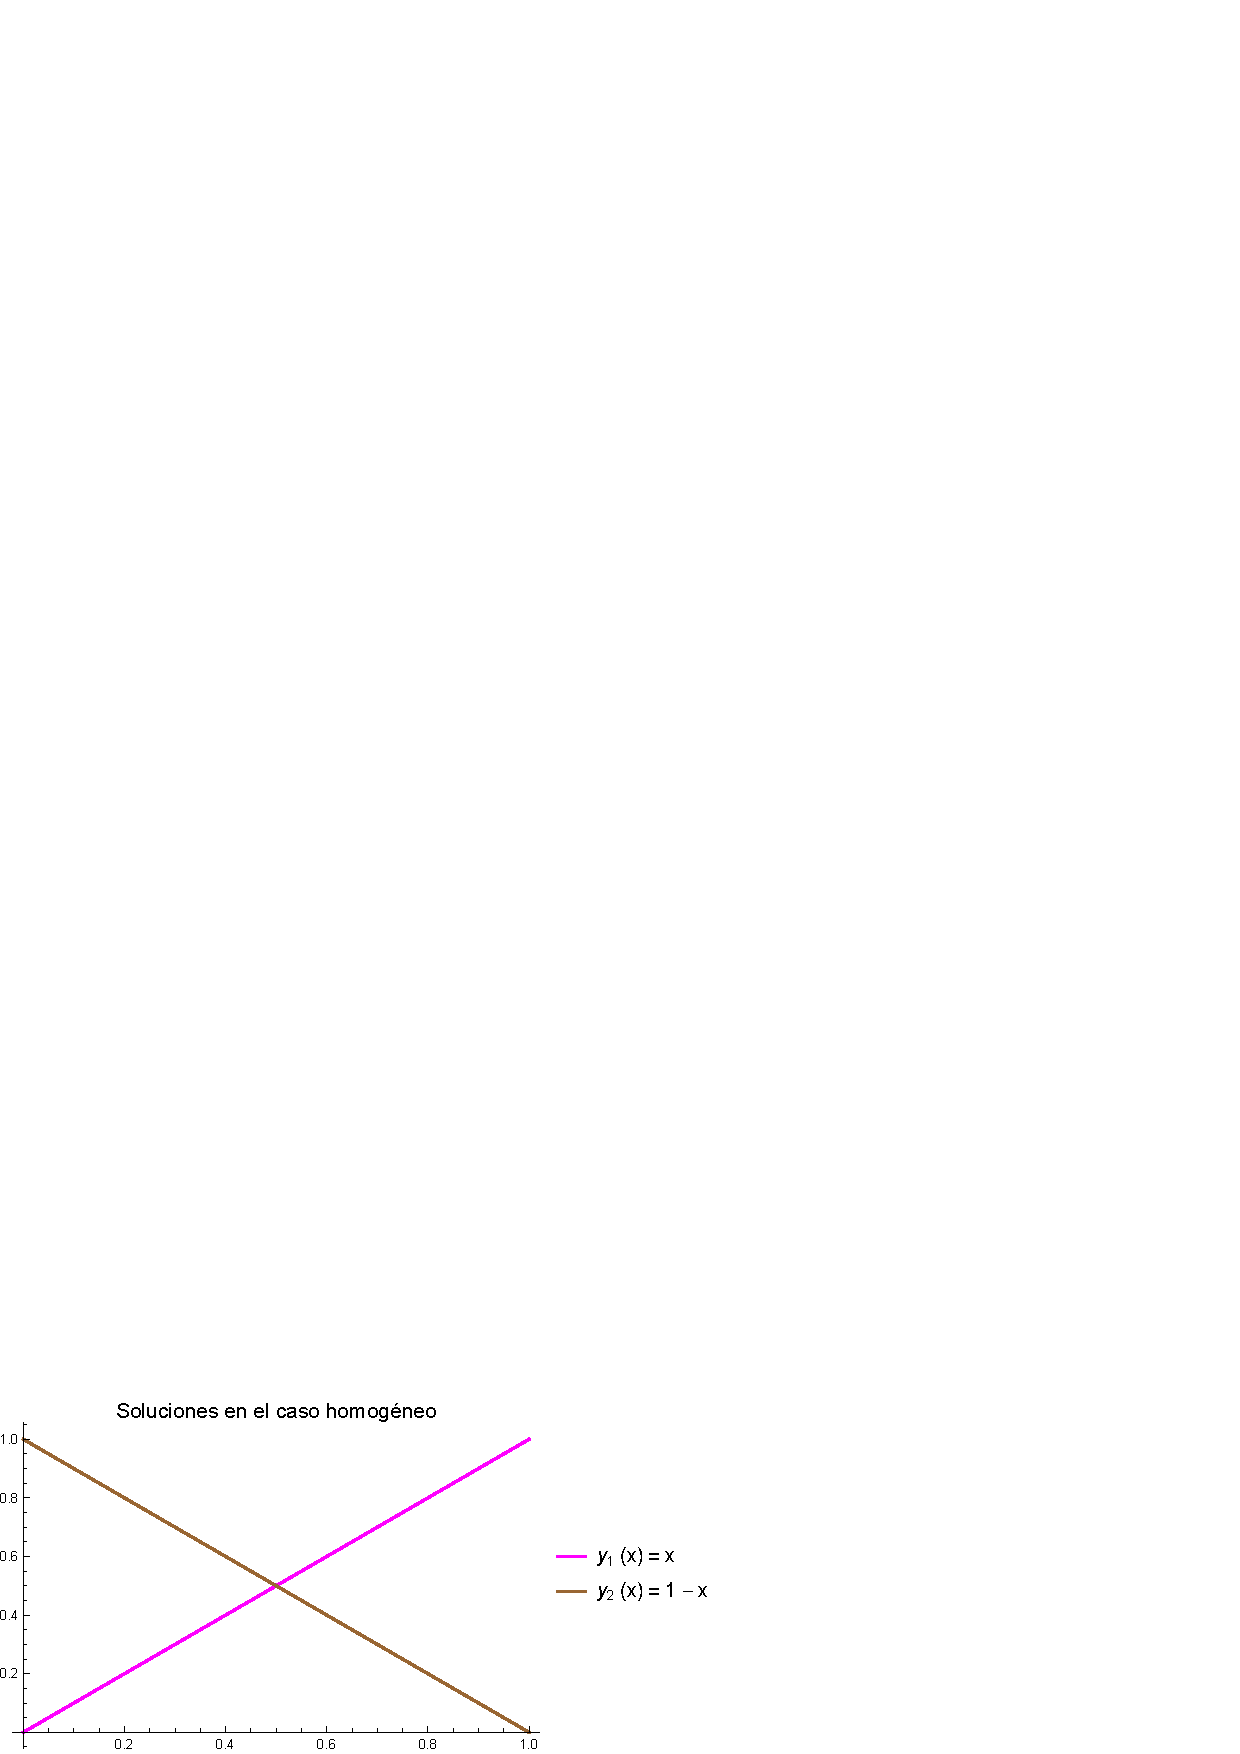
\includegraphics[scale=0.6]{Imagenes/Plot_EDONH_Green_01.pdf}
    \caption{Soluciones $y_{1} (x)$ y $y_{2} (x)$ para el caso de la ED homogénea.}
    \label{fig:figura_05}
\end{figure}
\end{frame}

\begin{frame}
\frametitle{Usando las soluciones}
Para este problema $p (x) = 1$. \pause Así, para $y_{1} (x) = x$ y $y_{2} (x) = 1 - x$, el producto:
\pause
\begin{eqnarray*}
\begin{aligned}
p (x) \, W (x) &=  y_{1} (x) \, \pderivada{y}_{2} (x) - \pderivada{y}_{1} (x) \, y_{2} (x) = \\[0.5em] \pause
&= x (-1) -  1(1 - x) = \\[0.5em] \pause
&= - 1
\end{aligned}
\end{eqnarray*}
Tomemos en cuenta que $p (x) \, W (x)$ es una constante, como debería ser.
\end{frame}

\begin{frame}
\frametitle{Obteniendo la función de Green}
Ahora construimos la función de Green.
\\
\bigskip
\pause
Así tenemos:
\pause
\begin{align}
G (x, \xi) = \begin{cases}
- \xi \, (1 - x), & 0 \leq \xi \leq x \\
- x \, (1 - \xi), & x \leq \xi \leq 1
\end{cases}
\label{eq:ecuacion_07_35}
\end{align}
\end{frame}

\begin{frame}
\frametitle{Simetría en la solución}
Observemos la simetría entre las dos partes de la función de Green. 
\\
\bigskip
\pause
Además, la función de Green satisface las CDF homogéneas: 
\pause
\begin{align*}
G (0, \xi) &= 0, \mbox{ de la parte inferior}, \\[0.5em]
G (1, \xi) &= 0, \mbox{ de la parte superior}
\end{align*}
\end{frame}

\begin{frame}
\frametitle{Forma integral}
Finalmente, sustituimos la función de Green en la forma integral de la solución y evaluamos la integral:
\pause
\begin{eqnarray*}
\begin{aligned}[b]
y (x) &= \scaleint{6ex}_{0}^{1} G (x, \xi) \, f (\xi) \dd{\xi} = \\[0.5em] \pause
&= \scaleint{6ex}_{0}^{1} G (x, \xi) \, \xi^{2} \dd{\xi} = \\[0.5em] \pause
&= - \scaleint{6ex}_{0}^{x} \xi \, (1 - x) \, \xi^{2} \dd{\xi} - \scaleint{6ex}_{x}^{1} x \, (1 - \xi) \, \xi^{2} \dd{\xi} = \\[0.5em]
\end{aligned}
\end{eqnarray*}
\end{frame}

\begin{frame}
\frametitle{Forma integral}
\begin{eqnarray}
\begin{aligned}[b]
&= - (1 - x) \scaleint{6ex}_{0}^{x} \xi^{3} \dd{\xi} - x \, \scaleint{6ex}_{x}^{1} (\xi^{2} - \xi^{3}) \dd{\xi} = \\[0.5em] \pause
&= - (1 - x) \bigg[ \dfrac{\xi^{4}}{4} \bigg] \eval_{0}^{4} - x \bigg[ \dfrac{\xi^{3}}{3} - \dfrac{\xi^{4}}{4} \bigg] \eval_{x}^{1} = \\[0.5em] \pause
&= \dfrac{1}{4} (1 - x) x^{4} - \dfrac{1}{12} \, x (4 - 3) + \dfrac{1}{12} \, x (4 x^{3} - 3 x^{4}) = \\[0.5em] \pause
&= \dfrac{1}{12} (x^{4} - x)
\end{aligned}
\label{eq:ecuacion_07_36}
\end{eqnarray}
\end{frame}

\begin{frame}
\frametitle{Solución a la ED}
Revisando la solución, se verifica fácilmente que la ED:
\pause
\begin{align*}
\sderivada{y} = x^{2}
\end{align*}
se satisface para las CDF $y (0) = 0$ y $y (1) = 0$. \pause La solución completa al caso no homogéneo se presenta en la figura (\ref{fig:figura_05}).
\end{frame}

\begin{frame}
\frametitle{Gráfica de la solución}
\begin{figure}[H]
    \centering
    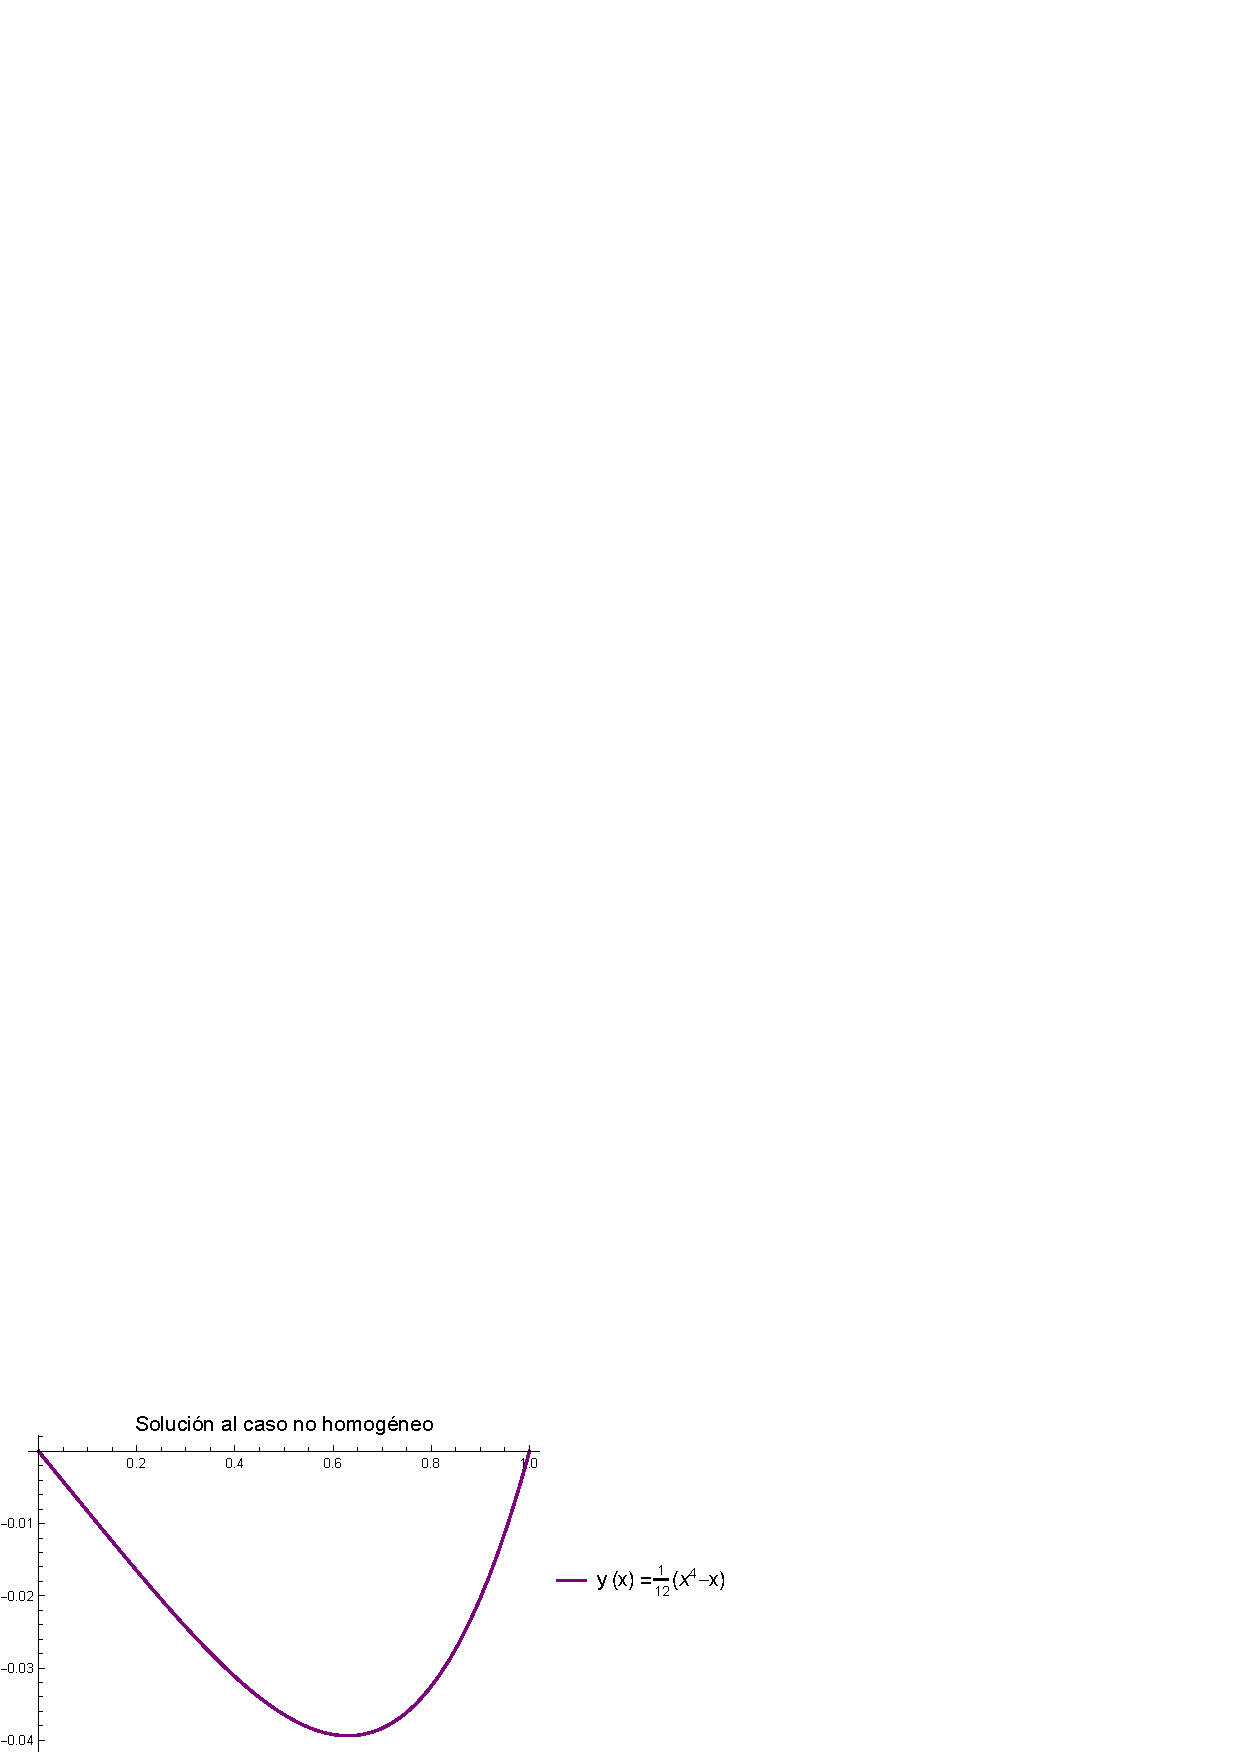
\includegraphics[scale=0.65]{Imagenes/Plot_EDONH_Green_02.pdf}
    \caption{Solución a la ED no homogénea que cumple con las CDF indicadas en el ejercicio.}
    \label{fig:figura_06}
\end{figure}
\end{frame}

\section{Propiedades de la función de Green}
\frame{\tableofcontents[currentsection, hideothersubsections]}
\subsection{Propiedades básicas}

\begin{frame}
\frametitle{Utilidad de las propiedades}
Hemos mencionado algunas propiedades de las funciones de Green en el último numeral.
\\
\bigskip
\pause
En esta parte revisaremos algunas de estas propiedades como una herramienta para construir rápidamente funciones de Green para problemas de valores en la frontera.
\end{frame}

\begin{frame}
\frametitle{Cinco propiedades}
\setbeamercolor{item projected}{bg=dartmouthgreen,fg=bisque}
\setbeamertemplate{enumerate items}{%
\usebeamercolor[bg]{item projected}%
\raisebox{1.5pt}{\colorbox{bg}{\color{fg}\footnotesize\insertenumlabel}}%
}
\begin{enumerate}[<+->]
\item \textbf{Ecuación Diferencial: } La función de Green con valor de frontera satisface la ED:
\pause
\begin{align*}
\pdv{x} \bigg[ p (x) \, \pdv{G (x, \xi)}{x} \bigg] + q (x) \, G (x, \xi) = 0, \hspace{0.5cm} x \neq \xi
\end{align*}
Esto se establece fácilmente. \pause Para $x < \xi$ estamos en el  segundo caso y $G (x, \xi)$ es proporcional a $y_{1} (x)$.
\seti
\end{enumerate}
\end{frame}

\begin{frame}
\frametitle{Cinco propiedades}
Así, dado que $y_{1} (x)$ es una solución de la ecuación homogénea, también lo es $G (x, \xi)$. Para $x > \xi$ estamos en el primer caso y $G (x, \xi)$ es proporcional a $y_{2} (x)$.
\\
\bigskip
\pause
Entonces, una vez más $G (x, \xi)$ es una solución del problema homogéneo.
\end{frame}

\begin{frame}
\frametitle{Cinco propiedades}
\setbeamercolor{item projected}{bg=dartmouthgreen,fg=bisque}
\setbeamertemplate{enumerate items}{%
\usebeamercolor[bg]{item projected}%
\raisebox{1.5pt}{\colorbox{bg}{\color{fg}\footnotesize\insertenumlabel}}%
}
\begin{enumerate}[<+->]
\conti
\item \textbf{CDF :} En el ejemplo del numeral anterior, se vio que $G (a, \xi) = 0$ y $G (b, \xi) = 0$.
\\
\bigskip
\pause
Por ejemplo, para $x = a$ estamos en el segundo caso y $G (x, \xi)$ es proporcional a $y_{1} (x)$.
\seti
\end{enumerate}
\end{frame}

\begin{frame}
\frametitle{Cinco propiedades}
Por lo tanto, cualquier condición que satisfaga $y_{1} (x)$, $G (x, \xi)$ la satisfará. Se puede hacer una afirmación similar para $x = b$.
\end{frame}

\begin{frame}
\frametitle{Cinco propiedades}
\setbeamercolor{item projected}{bg=dartmouthgreen,fg=bisque}
\setbeamertemplate{enumerate items}{%
\usebeamercolor[bg]{item projected}%
\raisebox{1.5pt}{\colorbox{bg}{\color{fg}\footnotesize\insertenumlabel}}%
}
\begin{enumerate}[<+->]
\conti
\item \textbf{Simetría o reciprocidad :} $G (x, \xi) = G (\xi, x)$. 
\\
\bigskip
\pause
Se demostró esta propiedad en el numeral anterior.
\seti
\end{enumerate}
\end{frame}

\begin{frame}
\frametitle{Cinco propiedades}
\setbeamercolor{item projected}{bg=dartmouthgreen,fg=bisque}
\setbeamertemplate{enumerate items}{%
\usebeamercolor[bg]{item projected}%
\raisebox{1.5pt}{\colorbox{bg}{\color{fg}\footnotesize\insertenumlabel}}%
}
\begin{enumerate}[<+->]
\conti
\item \textbf{Continuidad de $\mathbf{G}$ en $x = \xi$ :} $G (\xi^{+}, \xi) = G (\xi^{-}, \xi)$
\\
\bigskip
\pause
Aquí definimos $\xi^{\pm}$ a través de los límites de una función cuando $x$ tiende a $\xi$ desde arriba o desde abajo
\seti
\end{enumerate}
\end{frame}

\begin{frame}
\frametitle{Cinco propiedades}
En particular:
\pause
\begin{align*}
G (\xi^{+}, x) &= \lim_{x \uparrow \xi}, \hspace{0.4cm} x > \xi \\[0.5em]
G (\xi^{-}, x) &= \lim_{x \downarrow \xi}, \hspace{0.4cm} x < \xi
\end{align*}
\pause
Haciendo $x = \xi$ en ambos casos, tenemos que:
\pause
\begin{align*}
\dfrac{y_{1} (\xi) \, y_{2} (\xi)}{p \, W} = \dfrac{y_{1} (\xi) \, y_{2} (\xi)}{p \, W}
\end{align*}
\end{frame}

\begin{frame}
\frametitle{Cinco propiedades}
Por tanto, hemos establecido la continuidad de $G (x, \xi)$ entre los dos casos en $x = \xi$.
\end{frame}

\begin{frame}
\frametitle{Cinco propiedades}
\setbeamercolor{item projected}{bg=dartmouthgreen,fg=bisque}
\setbeamertemplate{enumerate items}{%
\usebeamercolor[bg]{item projected}%
\raisebox{1.5pt}{\colorbox{bg}{\color{fg}\footnotesize\insertenumlabel}}%
}
\begin{enumerate}[<+->]
\conti
\item \textbf{Salto de discontinuidad de $\displaystyle \pdv{G}{x}$ en $x = \xi$ :}
\pause
\begin{align*}
\pdv{G (\xi^{+}, \xi)}{x} - \pdv{G (\xi^{-}, \xi)}{x} = \dfrac{1}{p (\xi)}
\end{align*}
Esta propiedad no es tan obvia.
\seti
\end{enumerate}
\end{frame}

\begin{frame}
\frametitle{Cinco propiedades}
Primero calculamos las derivadas observando qué caso está involucrado y luego evaluamos las derivadas y las restamos.
\\
\bigskip
\pause
Así, tenemos lo siguiente:
\pause
\begin{eqnarray*}
\begin{aligned}[b]
&\pdv{G (\xi^{+}, \xi)}{x} - \pdv{G (\xi^{-}, \xi)}{x} = - \dfrac{1}{p \, W} \, y_{1} (\xi) \, \pderivada{y}_{2} (\xi) + \dfrac{1}{p \, W} \, \pderivada{y}_{1} (\xi) \, y_{2} (\xi) = \\[0.5em]
\end{aligned}
\end{eqnarray*}
\end{frame}

\begin{frame}
\frametitle{Cinco propiedades}
\begin{eqnarray}
\begin{aligned}[b]
&= - \dfrac{\pderivada{y}_{1} (\xi) \, y_{2} (\xi) - y_{1} (\xi) \, \pderivada{y}_{2} (\xi)}{p (\xi) \, \big[ y_{1} (\xi) \, \pderivada{y}_{2} (\xi) - \pderivada{y}_{1} (\xi) \, y_{2} (\xi) \big]} = \\[0.5em] \pause
&= \dfrac{1}{p (\xi)}
\end{aligned}
\label{eq:ecuacion_07_37}
\end{eqnarray}
\end{frame}

\begin{frame}[plain]
\begin{tcolorbox}[title={\centering Propiedades de la función de Green}]
\setbeamercolor{item projected}{bg=denim,fg=white}
\setbeamertemplate{enumerate items}{%
\usebeamercolor[bg]{item projected}%
\raisebox{1.5pt}{\colorbox{bg}{\color{fg}\footnotesize\insertenumlabel}}%
}
\begin{enumerate}[<+->]
\item \textbf{ED:}
\begin{align*}
\pdv{x} \bigg[ p (x) \, \pdv{G (x, \xi)}{x} \bigg] + q (x) \, G (x, \xi) = 0, \hspace{0.5cm} x \neq \xi
\end{align*}
\item \textbf{CDF: } Con cualesquiera condiciones $y_{1} (x)$ y $y_{2} (x)$ que se satisfagan, $G (x, \xi)$ se satisface.
\item \textbf{Simetría o reciprocidad :} $G (x, \xi) = G (\xi, x)$
\item \textbf{Continuidad de $\mathbf{G}$ en $x = \xi$ :} $G (\xi^{+}, \xi) = G (\xi^{-}, \xi)$
\seti
\end{enumerate}
\end{tcolorbox}
\end{frame}

\begin{frame}[plain]
\begin{tcolorbox}[title={\centering Propiedades de la función de Green}]
\setbeamercolor{item projected}{bg=denim,fg=white}
\setbeamertemplate{enumerate items}{%
\usebeamercolor[bg]{item projected}%
\raisebox{1.5pt}{\colorbox{bg}{\color{fg}\footnotesize\insertenumlabel}}%
}
\begin{enumerate}[<+->]
\conti
\item \textbf{Salto de discontinuidad de $\displaystyle \pdv{G}{x}$ en $x = \xi$ :}
\begin{align*}
\pdv{G (\xi^{+}, \xi)}{x} - \pdv{G (\xi^{-}, \xi)}{x} = \dfrac{1}{p (\xi)}
\end{align*}
\end{enumerate}
\end{tcolorbox}
\end{frame}

\subsection*{Ejercicio 3}

\begin{frame}
\frametitle{Enunciado del Ejecicio 3}
Construye la función de Green para el siguiente problema:
\pause
\begin{align*}
\sderivada{y} &+ \omega^{2} \, y = f(x) \hspace{0.6cm} 0 < x < 1 \\[0.5em]
&=y (0) = 0 = y (1) \hspace{0.6cm} \omega \neq 0
\end{align*}
\end{frame}

\begin{frame}
\frametitle{Procedimiento}
\setbeamercolor{item projected}{bg=eggplant,fg=white}
\setbeamertemplate{enumerate items}{%
\usebeamercolor[bg]{item projected}%
\raisebox{1.5pt}{\colorbox{bg}{\color{fg}\footnotesize\insertenumlabel}}%
}
\begin{enumerate}[<+->]
\item \textbf{Encontrar las soluciones a la ecuación homogénea.}
\pause
Una solución general a la ecuación homogénea está dada por:
\pause
\begin{align*}
y_{h} (x) = c_{1} \, \sin \omega x + c_{2} \, \cos \omega x
\end{align*}
\seti
\end{enumerate}
\end{frame}

\begin{frame}
\frametitle{Procedimiento Paso 1}
Por lo que, para $x \neq \xi$:
\pause
\begin{align*}
G (x, \xi) = c_{1} (\xi) \, \sin \omega x + c_{2} (\xi) \, \cos \omega x
\end{align*}
\end{frame}

\begin{frame}
\frametitle{Procedimiento}
\setbeamercolor{item projected}{bg=eggplant,fg=white}
\setbeamertemplate{enumerate items}{%
\usebeamercolor[bg]{item projected}%
\raisebox{1.5pt}{\colorbox{bg}{\color{fg}\footnotesize\insertenumlabel}}%
}
\begin{enumerate}[<+->]
\conti
\item \textbf{Condiciones de frontera.}
\pause
Primero, tenemos que $G (0, \xi) = 0$ para $0 \leq x \leq \xi$. Así:
\pause
\begin{align*}
G (0, \xi) = c_{2} (\xi) \, \cos \omega x = 0
\end{align*}
\pause
Entonces:
\pause
\begin{align*}
G (x, \xi) = c_{1} (\xi) \, \sin \omega x = 0, \hspace{0.5cm} 0 \leq x \leq \xi
\end{align*}
\seti
\end{enumerate}
\end{frame}

\begin{frame}
\frametitle{Procedimiento Paso 2}
Segundo, tenemos que $G (1, \xi) = 0$, para $\xi \leq x \leq 1$. Por lo tanto:
\pause
\begin{align*}
G (1, \xi) = c_{1} (\xi) \, \sin \omega + c_{2} (\xi) \, \cos \omega = 0
\end{align*}
\pause
Se puede elegir una solución haciendo que:
\pause
\begin{align*}
c_{2} (\xi) = - c_{1} (\xi) \, \tan \omega
\end{align*}
\end{frame}

\begin{frame}
\frametitle{Procedimiento Paso 2}
Esto nos proporciona:
\pause
\begin{align*}
G (x, \xi) = c_{1} (\xi) \, \sin \omega x - c_{1} (\xi) \, \tan \omega \, \cos \omega x
\end{align*}
\pause
Esto se puede simplificar factorizando el $c_{1} (\xi)$ y colocando los términos restantes sobre un denominador común.
\end{frame}

\begin{frame}
\frametitle{Procedimiento Paso 2}
El resultado es:
\pause
\begin{eqnarray}
\begin{aligned}[b]
G (x, \xi) &= \dfrac{c_{1} (\xi)}{\cos \omega} \big[ \sin \omega x \, \cos \omega - \sin \omega \, \cos \omega x \big] = \\[0.5em] \pause
&= - \dfrac{c_{1} (\xi)}{\cos \omega} \, \sin \omega (1 - x)
\end{aligned}
\label{eq:ecuaction_07_38}
\end{eqnarray}
\end{frame}

\begin{frame}
\frametitle{Procedimiento Paso 2}
Dado que el coeficiente es arbitrario en este punto, podemos escribir el resultado como:
\pause
\begin{align*}
G (x, \xi) = d_{1} (\xi) \, \sin \omega (1 - x), \hspace{0.5cm} \xi \leq x \leq 1
\end{align*}
\pause
Observamos que podríamos haber comenzado con $y_{2} (x) = \sin \omega (1 - x)$ como una de las soluciones linealmente independientes del problema homogéneo, anticipando que $y_{2} (x)$ satisface la segunda condición de frontera.
\end{frame}

\begin{frame}
\frametitle{Procedimiento Paso 3}
\setbeamercolor{item projected}{bg=eggplant,fg=white}
\setbeamertemplate{enumerate items}{%
\usebeamercolor[bg]{item projected}%
\raisebox{1.5pt}{\colorbox{bg}{\color{fg}\footnotesize\insertenumlabel}}%
}
\begin{enumerate}[<+->]
\conti
\item \textbf{Simetría o reciprocidad.}
\pause
Si imponemos que $G (x, \xi) = G (\xi, x)$. \pause En este punto tenemos que:
\pause
\begin{align*}
G (x, \xi) = \begin{cases}
c_{1} (\xi) \, \sin \omega x & 0 \leq x \leq \xi \\[0.5em]
d_{1} (\xi) \, \sin \omega (1 - x) & \xi \leq x \leq 1
\end{cases}
\end{align*}
\seti
\end{enumerate}
\end{frame}

\begin{frame}
\frametitle{Procedimiento Paso 3}
Podemos hacer que los casos sean simétricos eligiendo las formas correctas para $c_{1} (\xi)$ y $d_{1} (\xi)$. Elegimos :
\pause
\begin{align*}
c_{1} (\xi) &= C \, \sin \omega (1 - \xi) \\[0.5em]
d_{1} (\xi) &= C \, \sin \omega \xi
\end{align*}
\pause
Luego entonces:
\pause
\begin{align*}
G (x, \xi) = \begin{cases}
c_{1} (\xi) \, \sin \omega x & 0 \leq x \leq \xi \\[0.5em]
d_{1} (\xi) \, \sin \omega (1 - x) & \xi \leq x \leq 1
\end{cases}
\end{align*}
\end{frame}

\begin{frame}
\frametitle{Procedimiento Paso 3}
Ahora la función de Green es simétrica y todavía tenemos que determinar la constante $C$.
\\
\bigskip
\pause
Notemos que podríamos haber llegado a este punto usando el resultado del método de variación de parámetros donde $C = \dfrac{1}{p \, W}$.
\end{frame}

\begin{frame}
\frametitle{Procedimiento Paso 4}
\setbeamercolor{item projected}{bg=eggplant,fg=white}
\setbeamertemplate{enumerate items}{%
\usebeamercolor[bg]{item projected}%
\raisebox{1.5pt}{\colorbox{bg}{\color{fg}\footnotesize\insertenumlabel}}%
}
\begin{enumerate}[<+->]
\conti
\item \textbf{Continuidad de $G (x, \xi)$}.
\pause
Ya tenemos continuidad en virtud de la simetría impuesta en el último paso.
\seti
\end{enumerate}
\end{frame}

\begin{frame}
\frametitle{Procedimiento Paso 5}
\setbeamercolor{item projected}{bg=eggplant,fg=white}
\setbeamertemplate{enumerate items}{%
\usebeamercolor[bg]{item projected}%
\raisebox{1.5pt}{\colorbox{bg}{\color{fg}\footnotesize\insertenumlabel}}%
}
\begin{enumerate}[<+->]
\conti
\item \textbf{Salto de discontinuidad de $\displaystyle \pdv{x} G (x \xi)$}
\pause
Todavía necesitamos determinar $C$. Podemos hacer esto usando salto de discontinuidad en la derivada:
\pause
\begin{align*}
\pdv{G (\xi^{+}, \xi)}{x} - \pdv{G (\xi^{-}, \xi)}{x} = \dfrac{1}{p (\xi)}
\end{align*}
\end{enumerate}
\end{frame}

\begin{frame}
\frametitle{Procedimiento Paso 5}
En este problema $p (x) = 1$. Sustituyendo la función de Green, se tiene que:
\pause
\begin{eqnarray*}
\begin{aligned}[b]
1 & = \pdv{G (\xi^{+}, \xi)}{x} - \pdv{G (\xi^{-}, \xi)}{x} = \\[0.5em] \pause
&= \pdv{x} \big[ C \, \sin \omega (1 - x) \, \sin \omega \xi \big] \eval_{x = \xi} + \\[0.5em] \pause
&- \pdv{x} \big[ C \, \sin \omega (1 - \xi) \, \sin \omega \xi \big] \eval_{x = \xi} = 
\end{aligned}
\end{eqnarray*}
\end{frame}

\begin{frame}
\frametitle{Procedimiento Paso 5}
\begin{eqnarray}
\begin{aligned}[b]
&= - \omega \, C \, \cos \omega (1 - \xi) \, \sin \omega \xi - \omega \, C \, \sin \omega (1 - \xi) \, \cos \omega  \xi = \\[0.5em] \pause
&= - \omega \, C \, \sin \omega (\xi + 1 - \xi) = \\[0.5em] \pause
&= - \omega \, C \, \sin \omega
\end{aligned}
\label{eq:ecuacion_07_39}
\end{eqnarray}
\end{frame}

\begin{frame}
\frametitle{Procedimiento Paso 5}
Por lo tanto:
\pause
\begin{align*}
C = - \dfrac{1}{\omega \, \sin \omega}
\end{align*}
\end{frame}

\begin{frame}
\frametitle{Resultado esperado}
Finalmente, hemos obtenido la función de Green:
\pause
\begin{align}
G (x, \xi) = \begin{cases}
- \dfrac{\sin \omega (1 - \xi) \, \sin \omega x}{\omega \, \sin \omega} & 0 \leq x \leq \xi \\[1em]
- \dfrac{\sin \omega (1 - x) \, \sin \omega \xi}{\omega \, \sin \omega} & \xi \leq x \leq 1
\end{cases}
\label{eq:ecuacion_07_40}
\end{align}
\end{frame}

\end{document}